\documentclass[aoas,preprint]{imsart}
%\RequirePackage{mdframed}
%\usepackage{mdframed}
\usepackage[framemethod=TikZ]{mdframed}
\RequirePackage[OT1]{fontenc}
\usepackage[utf8x]{inputenc}
\RequirePackage{amsthm,amsmath}
\RequirePackage{natbib}
\RequirePackage[colorlinks,citecolor=blue,urlcolor=blue]{hyperref}

\usepackage[sc]{mathpazo}
\usepackage{amsmath, wrapfig}
\usepackage{dsfont}
\usepackage{graphicx}
\usepackage{caption}
\DeclareCaptionFormat{myformat}{\hrulefill \\ #1#2#3}
\DeclareCaptionFont{small}{\footnotesize}
\DeclareCaptionFont{blue}{\color{blue}} 
\DeclareCaptionFont{bf}{\bfseries}
\captionsetup[figure]{format=myformat,labelfont={blue,bf,small},font=small}
\usepackage{booktabs}% http://ctan.org/pkg/booktabs

%\usepackage{algorithm,algcompatible,amsmath}
\usepackage{algorithm, eqparbox,array}% http://ctan.org/pkg/algorithms
\usepackage{algpseudocode}% http://ctan.org/pkg/algorithmicx
%\usepackage{xcolor}
%\usepackage[usenames, dvipsnames]{color}
\usepackage{color}
\RequirePackage{xcolor}
%\usepackage{mdframed}




%\documentclass[11pt]{amsart}
%\usepackage{geometry,amsmath,amssymb,amsthm,cite,mathtools,float, caption, comment}                % See geometry.pdf to learn the layout options. There are lots.
%%\usepackage[numbers, sort&compress]{natbib}
%\usepackage[authoryear,sort]{natbib}
%\bibliographystyle{plainnat}
%\geometry{letterpaper}                   % ... or a4paper or a5paper or ... 
%%\geometry{landscape}                % Activate for for rotated page geometry
%%\usepackage[parfill]{parskip}    % Activate to begin paragraphs with an empty line rather than an indent
%\usepackage{graphicx}
%\usepackage{algorithm}
%\usepackage[noend]{algpseudocode}
%\usepackage{amssymb}
%\usepackage{epstopdf}
%\usepackage[parfill]{parskip}

 \setlength{\parskip}{1ex}
\newtheorem{lemma}{Lemma}
\newtheorem{theorem}{Theorem}
\newtheorem{prop}{Proposition}
\DeclareGraphicsRule{.tif}{png}{.png}{`convert #1 `dirname #1`/`basename #1 .tif`.png}

\begin{document}

\begin{frontmatter}
\title{A compositional model to assess expression changes from
 single-cell RNA-seq data}

\begin{aug}

\author{\fnms{Xiuyu} \snm{Ma}\thanksref{t1}\ead[label=e1]{ma79@wisc.edu}},
\author{\fnms{Keegan} \snm{Korthauer}\thanksref{k1}\ead[label=e2]{second@somewhere.com}},
\author{\fnms{Christina} \snm{Kendziorski}\thanksref{t2}\ead[label=e2]{kendzior@biostat.wisc.edu}},
\and
\author{\fnms{Michael} \snm{Newton}\thanksref{t1,t2}
\ead[label=e3]{newton@stat.wisc.edu}
\ead[label=u1,url]{http://www.foo.com}}

\affiliation{Department of Statistics\thanksmark{t1}, 
Department of Biostatistics and Medical Informatics\thanksmark{t2}, University of Wisconsin - Madison;
Dana Farber\thanksmark{k1} }

\address{Address of the First and Second authors\\
Usually a few lines long\\
\printead{e1}\\
\phantom{E-mail:\ }\printead*{e2}}

\address{Address of the Third author\\
Usually a few lines long\\
Usually a few lines long\\
\printead{e3}\\
\printead{u1}}


\end{aug}


\begin{abstract}
On the problem of scoring genes for evidence of changes in the distribution of single-cell expression, we
introduce a empirical Bayesian mixture approach and evaluate its operating characteristics 
in a range of numerical experiments.  The proposed approach leverages cell-subtype 
structure revealed in cluster analysis in order to boost gene-level information on expression changes.
Cell clustering informs gene-level analysis through a specially-constructed prior distribution
over pairs of multinomial probability vectors; this prior meshes with available model-based tools
that score patterns of differential expression over multiple subtypes.   
We derive an explicit formula for the posterior probability that a gene has the same distribution
in two cellular conditions, allowing for a gene-specific mixture over subtypes in each condition.
Advantage is gained by the compositional structure of the model, in which a host of gene-specific
mixture components are allowed, but also in which the mixing proportions are constrained at the whole 
cell level.  This structure leads to a novel form of information sharing through which the cell-clustering
results support gene-level scoring of differential distribution.  The result, according to our
numerical experiments, is improved sensitivity compared to several standard approaches
 for detecting distributional expression changes.  **plus connection to bursting and other**
\end{abstract}

%\maketitle
\end{frontmatter}

\section{Introduction}

The ability to measure genome-wide gene expression at single-cell resolution 
has accelerated the pace of biological discovery.  Overcoming data
analysis challenges caused by the scale and unique variation properties of single-cell
data will surely fuel further advances in immunology \citep{immune}, developmental
biology \citep{dv}, cancer \citep{cancer}, and other areas \citep{scs}. 
 Computational tools and statistical methodologies 
created for data of lower-resolution (e.g., bulk RNA-seq) or lower dimension 
(e.g., flow cytometry)  guide our response to 
 the data science demands of new measurement platforms,
but they remain inadequate for efficient knowledge discovery in this
rapidly advancing domain~\citep{Bacher2016}.

An important feature of single-cell studies that could be leveraged better
statistically is the fact that cells populate distinct, identifiable subtypes
determined by lineage history, epigenetic state, the activity
of various transcriptional programs, or other 
distinguishing factors. Extensive research on clustering cells
has produced tools for identifying subtypes, including: 
 \verb+SC3+ \citep{sc3}, \verb+CIDR+ \citep{CIDR} and \verb+ZIFA+ \citep{ZIFA}.
We hypothesize that such
subtype information may be usefully injected into other inference procedures in order
to improve their operating characteristics. 

Assessing the magnitude and statistical significance of changes in gene
expression associated with changes in cellular condition has been a central
statistical problem in genomics for which new tools specific to
the single-cell RNAseq data structure have been deployed: \verb+MAST+ \citep{ref:MAST},
\verb+SCDD+ \citep{ref:scDD}, \verb+D3E+ \citep{ref:d3e}, etc.  These tools respond
to scRNAseq characteristics, such as high prevelance of zero counts and
gene-level multimodality, but they do not fully exploit cellular-subtype
information.  We address this limitation, aiming to increase power to detect differential distribution.
The proposed method measures changes in a gene's marginal mixture distribution, and
acquires sensitivity  to a wide variety of distributional effects by how it integrates genome-wide with
gene-level data.  It is implemented in  software 
in the R package \textsc{scDDboost}, at \verb+http://github.com/wiscstatman/scDDboost/+.
Modularity in the necessary elements provides some methodological advantages. For example,
improvements in clustering, such as *sc3?*, may be used in place of the default clustering,
without altering the form of downstream analysis. **it's also relatively speedy computationally,
not requiring any MCMC**

Through the compositional model underlying \verb+scDDboost+, subtypes inferred by clustering 
inform the analysis of gene-level expression.  The proposed methodology merges two lines of computation
after cell clustering: one concerns patterns of differential expression among 
the cellular subtypes, and here we take advantage of the powerful \verb+EBseq+ method for detecting
patterns in negative-binomially-distributed expression data~\citep{ref:Leng}.  The second concerns 
the counts of cells in various subtypes; for this we propose a Double-Dirichlet-Mixture distribution
to model the pair of multinomial probability vectors for subtype counts in two experimental conditions.
Further elements are developed, on the selection of the number of subtypes and on accounting for uncertainty in the cluster output,  in order to provide an end-to-end solution to the differential distribution
problem.  

By way of example from  stem-cell biology,
Figure~\ref{fig:whet} shows data on several genes that are called by \verb+scDDboost+ to be
differentially distributed between two populations of cells. These particular genes
were not detected by other standard approaches (see Supplementary Material Section~1 for further details.)  
The proposed method is often better able to detect weak changes
compared to other methods, while at the same time 
agreeing with these methods on the strong differential signals and also not inflating the false-discovery rate. 
 **any more on these genes?**

\begin{figure}[H]
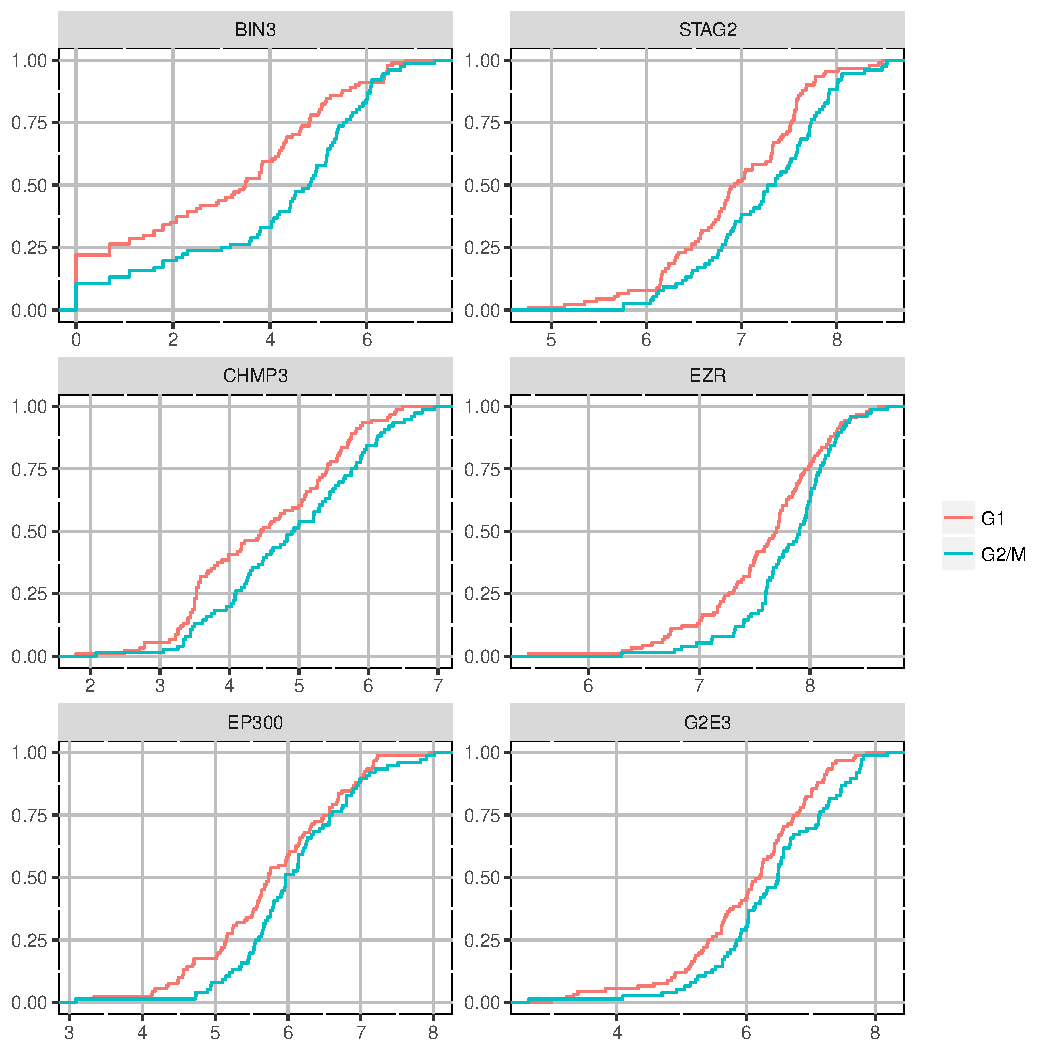
\includegraphics[width = 0.9\textwidth]{Figs/density_Fucci_dd.pdf}
 \caption{Cell cycle ralted genes uniquely identified by scDDboost
 from a study of stem cell differentiation (Leng {\em et al.} 2015). Shown are log2-scale expression
of  6 genes uniquely identified by scDDboost at 5\% FDR.  \label{fig:whet} }
\end{figure}




Numerical experiments  on both synthetic and published scRNA-seq data indicate that \verb+scDDboost+ has high
sensitivity for detecting subtle distribution changes. **link better with preceding paragraph*
  In these experiments we take advantage of
\verb+splatter+ for generating synthetic data~\citep{ref:Zappia} as well as the compendium of scRNA-seq
data available through \verb+conquer+ \citep{ref:Cq}.  **something on bursting?**
We also establish first-order asymptotic results for the methodology.    **any other results**

On organiziation, we present
the modeling and methodology elements in Section~2, numerical experiments in Section~3, and a discussion
in Section~4.  For presentation we move some details to an appendix and many others to a Supplementary 
Material document.



\section{Modeling}
\subsection{Data structure, sampling model, and parameters}

In modeling scRNASeq data, we
imagine that each cell $c$ falls into one of $K>1$ classes, which we think of as
subtypes or subpopulations of cells. For notation, $z_c=k$ means that cell $c$ happens to be of subtype $k$, with the vector $z=(z_c)$ recording
the states of all sampled cells.  Knowledge of this class structure
 prior to measurement is not required, as it will be inferred as necessary from
 available genomic data.   We expect that cells arise from multiple
experimental conditions, such as by treatment-control status or some other factors
 measured at the cell level, but we present our development for the special
case of two conditions.  Notationally, $y=(y_c)$ records the experimental condition, say $y_c=1$ or $y_c=2$.
 Let's say condition $j$ measures $n_j=\sum_{c} 1[y_c=j]$ cells,  and
in total we have $n=n_1+n_2$ cells in the analysis.  The examples in Section~3 involve hundreds to thousands of cells.
Further let \begin{eqnarray}
\label{eq:counts}
t^j_k = t^j_k(y,z) = \sum_c 1[y_c=j, z_c=k] 
\end{eqnarray}
denote the number of cells of subtype $k$ in condition $j$;
we infer something about these counts using genome-wide data.  As for molecular data, the 
normalized expression of gene $g$ in cell $c$, say $X_{g,c}$, is one entry
in a typically large {\sc{genes}} by {\sc{cells}} data matrix $X$.  Thus, the data structure entails an expression matrix
$X$, a treatment label vector $y$, and a vector $z$ of latent subtype labels.


We treat subtype counts in the two conditions,  $t^1 = (t^1_1, t^1_2, \cdots, t^1_K )$ and 
$t^2 = (t^2_1, t^2_2, \cdots, t^2_K)$,  as independent multinomial
vectors, reflecting the experimental design.  Explicitly,
\begin{eqnarray}
\label{eq:mult}
t^1| y \sim \text{Multinomial}_K( n_1, \phi ) \quad {\mbox {\rm and}} \quad
t^2| y \sim \text{Multinomial}_K( n_2, \psi )
\end{eqnarray}
for probability vectors 
$\phi = (\phi_1, \phi_2, \cdots, \phi_K)$ and 
 $\psi = ( \psi_1, \psi_2, \cdots, \psi_K)$ that characterize the populations of
cells from which the $n$ observed cells are sampled.  This follows from the more basic 
sampling model:
$P(z_c=k|y_c=1) = \phi_k$ and $P(z_c=k| y_c =2 ) = \psi_k.$

Our working hypothesis, referred to as the {\em compositional model},  is that any differences in the distribution of expression $X_{g,c}$ 
between $y_c=1$ and $y_c=2$ (i.e., any condition effects) are attributable 
to differences between the conditions 
in the underlying composition of cell types; i.e.,
owing to $\phi \neq \psi$.  We reckon that cells of any given subtype $k$ will
present data according to a distribution reflecting technical 
and biological variation specific to that class of cells, regardless of the 
condition the cell finds itself in.   Some care is needed in this, as an overly
broad cell subtype (e.g., {\em epithelial cells}) could have
further subtypes that show differential response to some treatment, for example,
and so cellular condition (treatment) would then affect the distribution of 
expression data within the subtype, which is contrary to our working hypothesis.
Were that the case,  we could have refined the subtype definition to allow a greater
number of population classes $K$ in order to mitigate the problem of within-subtype 
heterogeneity. A  risk in this approach is that $K$ could approach $n$, as if  
every cell were  its own subtype.  We find, however,
that data sets often encountered do not display this theoretical phenomenon
when considering a broad class of within-subtype expression distributions.
We revisit the issue in Section~4, but for now we proceed assuming 
that cellular condition affects the composition of subtypes but not the distribution of expression
within a subtype.

Within the compositional model, let $f_{g,k}$ denote the sampling distribution
of expression measurement $X_{g,c}$ assuming that cell $c$ is from subtype $k$.
Then for the two cellular conditions, and at some expression level $x$, 
the marginal distributions over subtypes are finite mixtures:
\begin{eqnarray*}
f_g^1(x) = \sum_{k=1}^K \phi_k f_{g,k} (x) \quad {\mbox {\rm and}} \quad
f_g^2(x) = \sum_{k=1}^K \psi_k f_{g,k} (x).
\end{eqnarray*}
In other words,  $X_{g,c} |[ y_c=j]  \sim f_g^j$  and $X_{g,c} |[ z_c=k, y_c=j] \sim f_{g,k}$.

We say that gene $g$ is {\em differentially distributed}, denote ${\rm DD}_g$ and indicated
$f_g^1 \neq f_g^2$,
if $f_g^1(x) \neq f_g^2(x)$ for some $x$, and otherwise it is equivalently distributed
(${\rm ED}_g$). Motivated by findings from bulk RNAseq data analysis, we further
set each $f_{g,k}$ to have a a negative-binomial form, say with mean $\mu_{g,k}$
and shape parameter $\sigma_g$; e.g. \cite{ref:Leng}, \cite{DES}, and \cite{ref:Des}. 
This choice is effective in our numerical experiments though it is 
not critical to the modeling formulation.  The use of mixtures per gene has proven
useful in related model-based approaches (e.g., Finak {\em et al.} 2015; McDavid {\em et al.} 2016;
Huang {\em et al.} 2018).
Our perspective is that  genome-wide data may usefully inform the  mixing proportions.

We seek methodology to prioritize genes for evidence
of ${\rm DD}_g$.  Interestingly, even if we have evidence for condition effects
on the subtype frequencies, it does not follow that a given
gene will have $f^1_g \neq f^2_g$; that depends on whether or not the subtypes
show the right pattern of {\em differential expression} at $g$, to use the 
standard terminology from bulk RNAseq.  For example, if two subtypes have 
different frequencies between the two conditions ($\phi_1 \neq \psi_1$ and 
 $\phi_2 \neq \psi_2$) but the same aggregate frequency
($\phi_1+\phi_2 = \psi_1 + \psi_2$),  and also  if $\mu_{g,1} = \mu_{g,2}$
then, other things being equal, $f^1_g = f^2_g$ even though $\phi \neq \psi$. The fact
is so central that we emphasize:


\noindent
{\bf Key issue:} A gene that does not distinguish two subtypes will also not distinguish
the cellular conditions if those subtypes appear in the same aggregate frequency
in the two conditions, regardless of changes in the individual subtype 
frequencies. 

 We formalize this issue in order that our methodology
has the necessary functionality.  To do so,  first consider the parameter space 
$\Theta = \{ \theta=(\phi, \psi,\mu, \sigma)  \}$,
where $\phi=(\phi_1, \phi_2, \cdots, \phi_K)$ and $\psi=(\psi_1, \psi_2, \cdots, \psi_K)$ 
are as before, where $\mu = \{ \mu_{g,k} \}$ holds  all the subtype-and-gene-specific expected
values, and where $\sigma = \{ \sigma_g \}$ holds all the gene-specific negative-binomial
shape parameters.  Critical to our construction are special subsets of $\Theta$ corresponding
to partitions of the $K$ cell subtypes.  A single partition, say $\pi$, is a set of
mutually exclusive and exhaustive blocks, $b$, say, each a subset of $\{1, 2, 
\cdots, K\}$, and we write $\pi = \{ b \}$.  Of course,
the set $\Pi$ containing all partitions $\pi$ of $\{1,2, \cdots, K\}$
 has cardinality that grows rapidly with $K$. 
 We carry along an example
involving $K=7$ cell types, and one three-block partition taken
from the set of 877 possible partitions of $\{1, 2, \cdots, 7\}$ (Figure 1).

\begin{figure}[h!]
  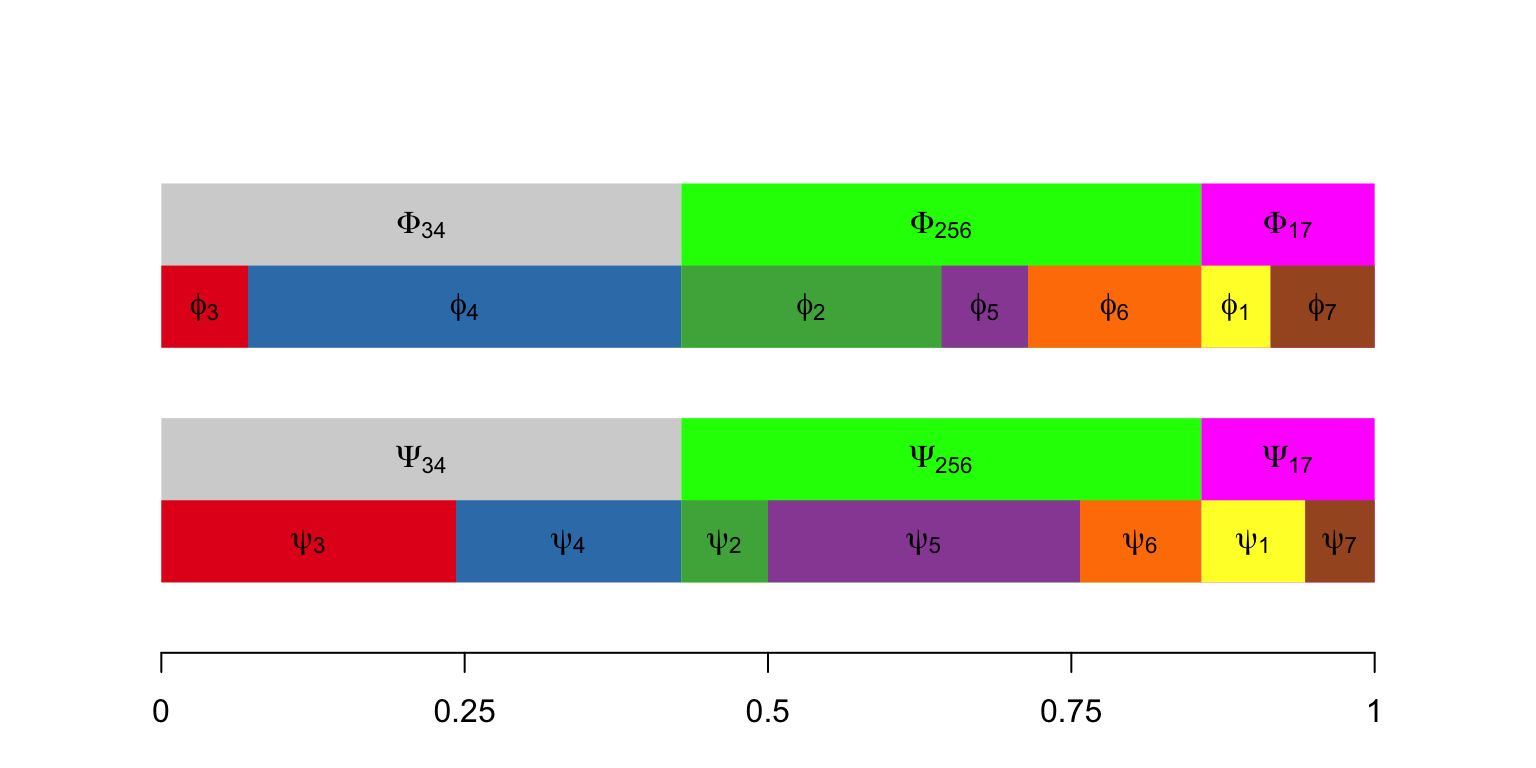
\includegraphics[width=\linewidth]{Figs/schematic-1.png}
  \caption{Proportions of $K=7$ cellular subtypes in different conditions. 
 Aggregated proportions of subtypes 3 and 4, subtypes 2, 5, and 6, and subtypes 1, and 7 
 remain same across conditions, while individual subtype frequencies change. 
 Depending on the changes in average expression among subtypes, these frequency changes
may or may not induce changes between two conditions  in the  marginal distribution of some gene's expression.  }
  \label{fig:1}
\end{figure}

%% Xiuyu, the alternative figure you had offered gives the suggestion that blocks of the
%% partition may need to be contiguous classes, which is not so...; with some other
%% stylistic differences, I decided to go back to the original; I realize your simulation
%% was not based on this one, but maybe that's ok


For any partition $\pi=\{b\}$, consider aggregate subtype frequencies
\begin{eqnarray*}
\Phi_b = \sum_{k\in b} \phi_k \quad {\mbox {\rm  and}} \quad 
 \Psi_b = \sum_{k\in b} \psi_k,
\end{eqnarray*}
and extend the notation, allowing vectors $\Phi_\pi = \{ \Phi_b: b \in \pi \}$ and similarly
for $\Psi_\pi$. Recall the partial ordering of partitions based on refinement, and note that
as long as $\pi$ is not the most refined partition (every cell type its own block),
then the mapping from $( \phi, \psi )$ to $( \Phi_\pi, \Psi_\pi)$ is many-to-one.
Further, define sets
\begin{eqnarray}
\label{eq:asets}
A_\pi = \{ \theta\in \Theta: \; \Phi_b = \Psi_b  \, \forall b \in \pi \}.
\end{eqnarray}
and
\begin{eqnarray}
\label{eq:msets}
M_{g,\pi} = \{ \theta \in \Theta: \; \mu_{g,k} = \mu_{g,k'} \iff k,k' \in b, b \in \pi \}.
\end{eqnarray}
Under $A_\pi$ there are constraints on cell subtype frequencies; under $M_{g,\pi}$ there is 
equivalence in the gene-level distribution of expression between certain subtypes.
These sets are precisely the
structures needed to address differential distribution DD$_g$ (and
it complement, equivalent distribution, ${\rm ED}_g$) at a given gene
$g$, since:

\begin{theorem}  Let $C_{g,\pi} = A_\pi\cap M_{g, \pi}$.  For 
partitions $\pi_1 \neq\pi_2$, \mbox{$C_{g,\pi_1} \cap C_{g,\pi_2} = \emptyset$}. Further,
 at any gene $g$, equivalent distribution is
\begin{eqnarray*}
{\rm{ED}}_g = \bigcup_{\pi \in \Pi} C_{g,\pi}.
\end{eqnarray*}
\end{theorem}
With additional 
probability structure on the parameter space,  we immediately obtain from Theorem~1 
a formula for local false discovery rates:
\begin{align}
\label{eq:lfdr}
1-P(\text{DD}_g|X,y) = 
 P(\text{ED}_g|X,y) = \sum_{\pi \in \Pi} P\left(A_\pi \cap M_{g,\pi} |X,y \right).
\end{align}
Such local false discovery rates are important empirical Bayesian 
statistics in large-scale testing (e.g., Efron, 2007; Muralidharan, 2010; Newton 
{\em et al.} 2004).  For example, the conditional false discovery rate of a list of genes 
is the arithmetic mean of the associated local false discovery rates.  
The partition representation guides construction of a prior distribution (Section 2.3) and a 
model-based method (Section 2.2) for scoring  differential distribution.   Setting the stage, 
Figure~2 shows the dependency structure of 
the proposed compositional model and the partition-reliant prior specification.

\begin{figure}[h!]
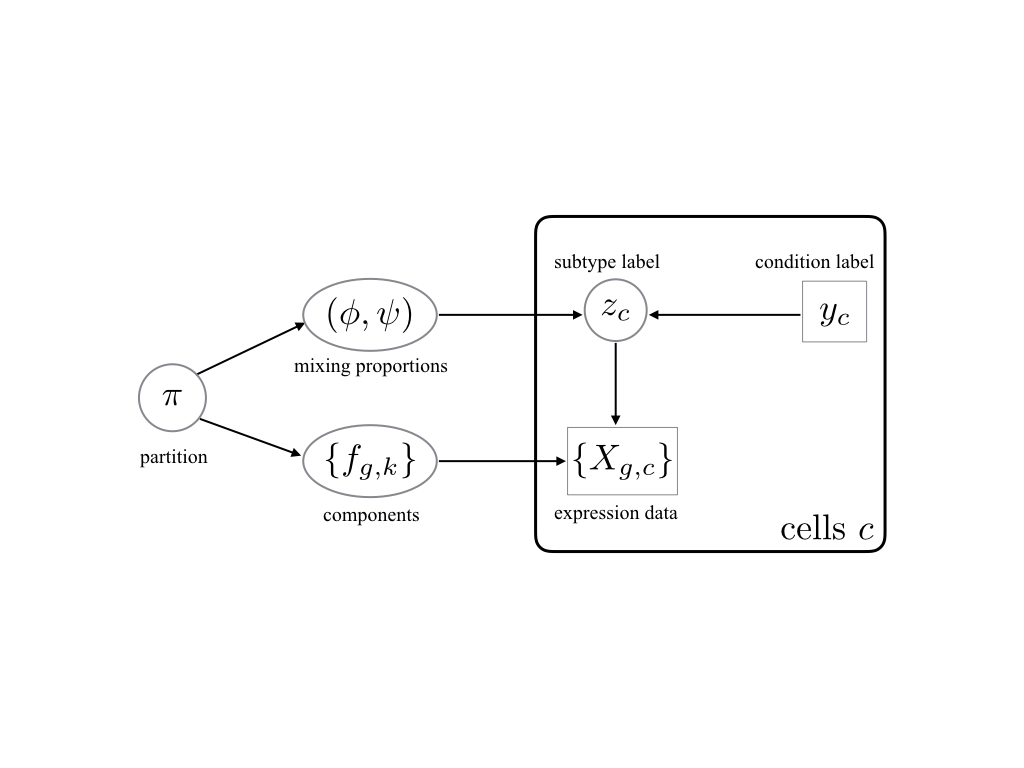
\includegraphics[trim={4cm 6cm 4cm 6cm}, clip, width=5in]{Figs/dag.png}
  \caption{Directed acyclic graph structure of compositional 
model and partition-reliant prior. The plate on the right side indicates i.i.d.
copies over cells $c$, conditionally on mixing proportions and mixing components.
 Observed data are indicated in rectangles/squares, and unobserved variables
are in circles/ovals. }
  \label{fig:2}
\end{figure}

Key to computing the gene-specific 
local false discovery rate $P(\text{ED}_g|X,y)$ is
evaluating probabilities $P\left(A_\pi \cap M_{g,\pi} |X,y \right)$ for
any subtype partition $\pi$ and gene $g$.
The dependence structure (Figure~2) implies a useful reduction of this
quantity, at least conditionally upon subtype labels $z=(z_c)$.

\begin{theorem}  
$  P\left(A_\pi \cap M_{g,\pi} |X,y,z \right) 
  =  P\left(A_\pi |y,z \right) \, 
                      P\left(M_{g,\pi}| X,z \right).  $
\end{theorem}

In what follows, we develop the  modeling and computational elements necessary  to efficiently evaluate inference summaries~(\ref{eq:lfdr}) taking advantage of 
Theorems~1 and~2.  Roughly, the methodological idea is that subtype labels $z$
have relatively low uncertainty, and may be estimated from genome-wide 
clustering of cells in the absence of condition information $y$ (up to an arbitrary label permutation). 
The modest bit of uncertainty in $z$
we handle through a computationally efficient randomized clustering scheme.
 Theorem~2 indicates that our computational task then separates into
two parts given $z$.  On one hand, cell subtype frequencies 
combine with condition labels to give
$P\left(A_\pi |y,z \right)$. Then gene-level data
locally drive the posterior probabilities $P\left(M_{g,\pi}| X,z \right)$ that
measure differential expression between subtypes. 
Essentially, the model provides a specific form of information 
sharing between genes  that leverages the compositional structure of single-cell 
data in order to sharpen our assessments of between-condition expression changes. 


\subsection{Method structure and clustering}

We leverage the extensive research on how to cluster cells into subtypes using scRNA-seq data:
for example,  SC3~\citep{sc3}, CIDR~\citep{CIDR}, and ZIFA~\citep{ZIFA}.   We propose clustering on the full set
of profiles in a way that is blind to the condition label vector $y$, in order to have as many cells as possible
to inform the subtype structure.  We investigated several clustering schemes in numerical experiments and allow 
flexibility in this choice within the \textsc{scDDboost} software. 
Associating clusters with subtype labels $\hat z_c$  estimates
the actual subtypes $z_c$, and prepares us to use Theorems~1 and~2 in order to compute separate
posterior probabilities $P(A_\pi|y, \hat z)$ and $P(M_{g, \pi}| X, \hat z)$ that are necessary for scoring
differential distribution. The first probability concerns patterns of cell counts over subtypes in the two conditions,
and has a convenient closed form within the double-Dirichlet model (Section~2.3).
The second probability concerns patterns of changes in expected expression levels among subtypes, and this is
also conveniently computed for negative-binomial counts using \textsc{EBSeq} \citep{ref:Leng}. 
Algorithm~\ref{alg:scDDcore}
summarizes how these elements combine to get the posterior probability of differential distribution per gene,
conditional on an estimate of the subtype labels.


%Our approach take transcripts processed by normalizing methods (e.g. SCnorm \cite{ref:Rhonda}). 
%The workflow contains two parts, classify cells into subtypes and posterior inference on distributional change. In the first part, recall subtype is a group of cells with distributions of transcripts that are specific to this group, regardless which condition the cells is from. Thus classification process is blind to conditions and can be done by clustering upon similarities between cells(supplementary material). 

\begin{algorithm}
\caption{\textsc{scDDBoost-core}}\label{alg:scDDcore}
\raggedright\hspace*{\algorithmicindent} \textbf{Input}: \begin{list}{}{}
 \item \textsc{genes} by \textsc{cells} expression data matrix $X=(X_{g,c})$
 \item  cell condition labels $y=(y_c)$ 
 \item  cell subtype labels (estimated)  $\hat z=(\hat z_c)$
 \end{list}
\hspace*{\algorithmicindent} 
\textbf{Output}:  posterior probabilities of differential distribution from estimated subtypes
\begin{algorithmic}[1]
\Procedure{scDDBoost-core}{$X,y,\hat z$}
 \item  number of cell subtypes $K = \rm{length}( \rm{unique}( \hat z ) )$  
\State subtype differential expression: $\forall g,\pi$ compute  $P(M_{g,\pi} | X, \hat z)$ using \verb+EBSeq+
\State cell frequency changes: $\forall \pi$ compute  $P(A_\pi | y, \hat z)$ using Double Dirichlet model 
\State posterior probability: $\forall g,  \, P(\text{ED}_g | X, y, \hat z)\gets \underset{\pi}{\sum}P(M_{g,\pi} | X, \hat z) \,
 P(A_\pi | y, \hat z)$
\State \textbf{return} $\forall g, \, P(\text{DD}_g |X, y, \hat z)=1-P(\text{ED}_g| X,y, \hat z)$
\EndProcedure
\end{algorithmic}
\end{algorithm}



%%One advantage of our approach is that the posterior inference can be incorporate with different clustering methods. With the development of technology, clustering methods taking care of newly discovered characteristic of scRNA seq data (e.g. SC3\cite{sc3}, CIDR\cite{CIDR} and ZIFA\cite{ZIFA}) could be substituted with our default one. No matter what clustering method is used, we estimate the mixture structure utilizing the whole genome information rather than estimating a gene specific mixture structure solely using information of that gene. Due to this reason, our model is more capable of capturing characteristic of scRNA seq data than scDD and we name our approach \textsc{scDDboost}. 

We invoke $K-$medoids \citep{kmedoids} 
as the default clustering method in \textsc{scDDboost}, and customize the cell-cell distance by integrating two measures.  
The first assembles gene-level information by cluster-based-similarity partitioning~\citep{ref:cspa}.
 Separately at each gene,   modal clustering (\cite{ref:dahl} and Appendix B) partitions the cells, and
then we define dissimilarity between cells as the mahattan distance of those gene specific partition labels.
A second measure defines dissimilarity by one minus the 
Pearson correlation between cells, which is computationally inexpensive,
less sensitive to outliers than Euclidean distance, and effective at detecting cellular clusters in 
scRNA-seq~\citep{Cor}.
 We combine the two measures by a weighted average, 
with  $w_C = \frac{\sigma_P}{\sigma_C + \sigma_P}$ and $w_P = 1 - w_C$. where $w_C,\sigma_C, w_P, \sigma_P$ are the weights and standard deviations of cluster-based distance and Pearson-correlation distance, respectively.
The final distance matrix is denoted $D=\left( d_{i,j} \right)$. 

Any clustering method  entails classification errors, and so $\hat z_c \neq z_c$ for some cells. To mitigate
the effects of this uncertainty, \textsc{scDDboost} averages output probabilities from \textsc{scDDboost-core} over
randomized clusterings $\hat z^*$.  These are not uniformly random, but rather are generated by applying $K-$medoids
to a randomized distance matrix $D^*=\left( d_{i,j}\times w_{i,j}\right)$, 
where $w_{i,j}$ are  unit mean, non-negative weights
$w_{i,j} = 1/( e_i + e_j )$, and where $( e_i) $ are independent and identically Gamma$(\hat a, \hat b)$ distributed
deviates for hyper-parameters $(\hat a, \hat b)$ derived from $D$.   We argue that the distribution of
clusterings induced by this simple computational 
scheme approximates a Bayesian posterior analysis (Supplementary Material
Section **).   Pseudo-code for the resulting \textsc{scDDboost} is in Algorithm~\ref{alg:scDDboost} (Appendix).
Averaging this way gives additional stability to the posterior probability statistics (Supplementary Material
Section **).


Computations become more intensive the larger is the number $K$ of cell subtypes. We also observe 
that  taking $K$ to be too large may inflate the false positive rate (Figure **).  The approach
taken in \verb+scDDboost+ is to set $K$ using the validity score~\citep{selK}, which measures 
changes in within-cluster sum of squares as we increase $K$.  Our specific implementation is in
Supplementary Material Section *.

%%Although there are various options for clustering methods, none of them guarantee the accuracy and posterior inference of differential distributed genes can be sensitive to the initial partition. Here we provide a method to make our inferences robust to partitions. Given number of subtypes $K$, the final posterior probabilities is obtained by averaging results from iterative run of \textsc{scDDboost-core}  with randomly generated subtype labels $z^*$. Taking account of information contained in $D = dist(X)$ , instead of purely random assigning subtype labels, we generate the distance matrices of cells $D^*$ by dividing weights to the original one and assign labels based on $D^*$. Specifically,  we random sample a noise vector $e$ with length equal to number of cells and components are i.i.d. gamma distributed,  then constructing the weighting matrix $W$ by $W_{i,j} = e_i + e_j$ and random distance matrix is obtained by $D^* = D /  W$(division is performed componentwisely).  The choice of gamma distributed weights and dividing transformation is to matched the probability of two units classified into the same group under random weighting to bayesian framework (supplementary material). 


%In simulations, 
%we observed that averaged adjusted Rand index as well as Rand index of mode of partitions based on randomized distance matrices is higher (better estimation) than that of partition based on original distance matrix (Supplementary Material, **?**). 
%{\em MAN to XM: please clarify}


\subsection{Double Dirichlet Mixture (DDM)}


%** ON THE PRIOR INDEPENDENCE**
%This expresses the idea that  subtype proportions $(\phi,\psi)$ are
%uninformative about the mean expression levels   $\{\mu_{g,i}\}$). Under this assumption:
%**


Here we describe the partition-reliant prior $p(\phi,\psi)$ indicated in~Figure~2 and derive an explicit
formula for $P(A_\pi|y,z)$.   We lose no generality here by defining
$A_\pi = \{ (\phi,\psi): \Phi_b = \Psi_b \;  \forall b \in \pi \}$, rather than as a subset of the full
parameter space as in~(\ref{eq:asets}).   Each $A_\pi$ is closed and convex subset of the product space
holding all possible pairs of length-$K$ probability vectors.

We propose a spike-slab-style mixture prior with the following form:
\begin{eqnarray}
\label{eq:ddmix}
p(\phi,\psi) = \sum_{\pi \in \Pi} \omega_\pi  \, p_\pi(\phi,\psi ).
\end{eqnarray} 
Each mixture component $p_\pi(\phi,\psi)$ has support $A_\pi$;  
the mixing proportions $\omega_\pi$ are any non-negative constants summing to one. 
To specify component $p_\pi$,  notice that on $A_\pi$ there is a 1-1 correspondence between pairs $(\phi, \psi)$ and 
parameter states:
\begin{eqnarray}
\label{eq:onetoone}
 \left\{ (\tilde \phi_b, \tilde \psi_b, \Phi_b), \; \forall b \in \pi \right\}, 
\end{eqnarray}
where
\begin{eqnarray*}
\tilde{\phi}_b = \frac{\phi_b}{\Phi_b}, \quad \tilde{\psi}_b = \frac{\psi_b}{\Psi_b}, \quad 
{\mbox {\rm and}} \quad \Phi_b = \sum_{k \in b} \phi_k = \sum_{k \in b} \psi_k = \Psi_b.
\end{eqnarray*}
For example, $\tilde{\phi}_b$ is a vector of conditional probabilities for each subtype given that a cell
from the first condition is one of the subtypes in $b$. 


We introduce hyperparameters
$\alpha^1_k, \alpha^2_k>0$ for each subtype $k$, and set 
$\beta_b = \sum_{k \in b}\left( \alpha^1_k + \alpha^2_k \right)$ for any possible block $b$.
Extending notation, let $\alpha_b^j$ be the vector of $\alpha_k^j$
for $k\in b$, $\beta_\pi$ be the vector of $\beta_b$ for $b \in \pi$, $\phi_b$ and $\psi_b$ be vectors
of $\phi_k$ and $\psi_k$, respectively, for $k\in b$, and $\Phi_\pi$ and $\Psi_\pi$ be the vectors
of $\Phi_b$ and $\Psi_b$ for $b \in \pi$.  The proposed double-Dirichlet component 
$p_\pi$ is determined in the transformed scale by assuming $\Psi_\pi = \Phi_\pi$ and further:
\begin{eqnarray}
\label{eq:doubledir}
\Phi_\pi  &\sim& \text{Dirichet}_{N(\pi)}[   \beta_\pi   ]  \\ \nonumber
\tilde \phi_b  &\sim & \text{Dirichlet}_{N(b)}[ \alpha_b^1 ] \qquad \forall b \in \pi \\ \nonumber
\tilde \psi_b  &\sim & \text{Dirichlet}_{N(b)}[ \alpha_b^2 ] \qquad \forall b \in \pi 
\end{eqnarray}
where $N(\pi)$ is the number of blocks in $\pi$ and $N(b)$ is the number of subtypes in $b$, and
where all random vectors in~(\ref{eq:doubledir}) are mutually independent.  
Mixing over $\pi$ as in~(\ref{eq:ddmix}), we write
$(\phi,\psi) \sim {\mbox {\rm DDM}}\left[ \omega=(\omega_\pi),
\alpha^1=(\alpha^1_k), \alpha^2 = (\alpha^2_k) \right].$


We record some properties of the component distributions $p_\pi$:
%%using the well-known Dirichlet-multinomial conjugacy and the Dirichlet collapsing property~\citep{ref:Dickey}. 

\noindent
{\bf Property 1:}  In $p_\pi(\phi,\psi)$, $\psi$ and $\phi$ are dependent, unless $\pi$ is the null 
partition in which all subtypes constitute a single block.

%\noindent
%{\bf Property 2:}  If $\alpha^1=\alpha^2$, then both $\phi$ and $\psi$ are marginally distributed
%as Dirichlet$_K(\alpha^1)$.  

\noindent
{\bf Property 2:} With $k \in b$, marginal means are:
\begin{eqnarray*}
E_\pi\left( \phi_k \right ) = \frac{ \alpha^1_k }{ \sum_{k' \in b} \alpha^1_{k'} } \,
		\frac{ \beta_b }{ \sum_{b' \in \pi} \beta_{b'} } \quad {\mbox {\rm and}} \quad
E_\pi\left( \psi_k \right ) = \frac{ \alpha^2_k }{ \sum_{k' \in b} \alpha^2_{k'} }  \,
		\frac{ \beta_b }{ \sum_{b' \in \pi} \beta_{b'} } .
\end{eqnarray*}

Recall from~(\ref{eq:counts}) the vectors $t^1$ and $t^2$ holding
counts  of cells in each subtype in each condition, computed from $y$ and $z$.  Relative to a block $b \in \pi$, 
let $t^j_b = \sum_{k\in b} t^j_k$, for cell conditions $j=1,2$, and,
let $t^j_\pi$ be the vector of these counts over $b \in \pi$.   The following properties refer to
marginal distributions in which $(\phi,\psi)$ have been integrated out of the joint
distribution involving~(\ref{eq:mult}) and the component $p_\pi$.

\noindent
{\bf Property 3:}  $t^1$ and $t^2$ are conditionally independent given $y$, $t^1_\pi$ and $t^2_\pi$.

\noindent
{\bf Property 4:}  For $j=1,2$,
\begin{eqnarray*}
p_\pi(t^j | t^j_{\pi},y) = \prod_{b \in \pi} \left\{
\left[ \frac{ \Gamma(t^j_b +1 ) }{\prod_{k \in b} \Gamma( t^j_k + 1 ) } 
\right]
\left[ \frac{\Gamma( \sum_{k \in b} \alpha_k^j )}{
		\prod_{k\in b} \Gamma( \alpha_k^j ) } \right] 
       \left[        \frac{ \prod_{k \in b} \Gamma(\alpha_k^j + t^j_k)  }{
		\Gamma(t^j_b + \sum_{k\in b} \alpha_k^j ) )}\right]
 \right\}
\end{eqnarray*}

\noindent
{\bf Property 5:}  
\begin{eqnarray*}
p_\pi(t^1_{\pi},t^2_{\pi}| y) =
 \left[ \frac{ \Gamma(n_1+1) \Gamma(n_2+1) }{ \prod_{b \in \pi} \Gamma(t^1_b+1) 
   \Gamma( t^2_b + 1 )} \right] 
\left[ \frac{\Gamma( \sum_{b \in \pi} \beta_b  )}{
   \prod_{b \in \pi} \Gamma(\beta_b )} \right] 
 \left[ \frac{ \prod_{b \in \pi} \Gamma( \beta_b + t^1_b + t^2_b )}{
	\Gamma( n_1 + n_2 + \sum_{b \in \pi} \beta_b  )} \right].
\end{eqnarray*}


Let's look at some special cases to dissect this result. 

Case 1. If $\pi$ has a single block equal to the entire
 set of cell types $\{1,2, \cdots, K\}$,  then $t^j_b=n_j$ for both $j=1,2$,
and Property~5 reduces, correctly, to 
$p_\pi(t^1_{\pi},t^2_{\pi}| y) = 1$.  Further,
\begin{eqnarray*}
p_\pi(t^j | t^j_{\pi},y) = 
\left[ \frac{ \Gamma(n_j +1 ) }{ \Gamma( n_j + \sum_{k=1}^K \alpha_k^j ) }
\right]
\left[ \frac{\Gamma( \sum_{k =1}^K \alpha_k^j )}{
                \prod_{k=1}^K \Gamma( \alpha_k^j ) } \right]
       \left[    \prod_{k=1}^K    \frac{  \Gamma(\alpha_k^j + t^j_k)}{
                \Gamma(t^j_k + 1 )}\right]
\end{eqnarray*}
which is the well-known Dirichlet-multinomial predictive distribution
for counts $t^j$~\citep{Wag}.  E.g, taking $\alpha_k^j=1$ for all types $k$ 
we get the uniform distribution
\begin{eqnarray*}
p_\pi(t^j | t^j_{\pi},y) = 
 \frac{ \Gamma(n_j +1 ) \Gamma(K) }{ \Gamma( n_j + K ) }.
\end{eqnarray*}

Case 2. At the opposite extreme, $\pi$  has one block $b$ for each
 class $k$, so $\phi=\psi$. Then $p_\pi(t^j | t^j_{\pi},y) = 1$, and 
further, writing $b = k$,
\begin{eqnarray*}
p_\pi(t^1_{\pi},t^2_{\pi}|y ) =
 \left[ \frac{ \Gamma(n_1+1) \Gamma(n_2+1) }{ \prod_{k=1}^K 
   \Gamma(t^1_k+1) 
   \Gamma( t^2_k + 1 )} \right] 
\left[ \frac{\Gamma( \sum_{k=1}^K \beta_k  )}{
   \prod_{k=1}^K \Gamma(\beta_k)} \right] 
 \left[ \frac{ \prod_{k=1}^K \Gamma( \beta_k + t^1_k + t^2_k )}{
	\Gamma( n_1 + n_2 + \beta_k  )} \right].
\end{eqnarray*}
which corresponds to Dirichlet-multinomial predictive distribution for counts $t^1 + t^2$ 
since $t^1$ and $t^2$ are identical distributed given $(\phi,\psi)$ in this case.


The properties above are useful in establishing:
\begin{theorem}
The DDM model is conjugate to multinomial sampling of $t^1$ and $t^2$:
\begin{eqnarray*}
(\phi,\psi)|y,z  \sim {\mbox {\rm DDM}}\left[ \omega^{\rm post}=(\omega^{\rm post}_\pi), \alpha^1 + t^1, \alpha^2 + t^2  \right]
\end{eqnarray*}
where
\begin{eqnarray*}
\omega^{\rm post}_\pi \propto 
 p_\pi(t^1 | t^1_{\pi},y)\, p_\pi(t^2|  t^2_{\pi},y )
 \, p_\pi( t^1_{\pi}, t^2_{\pi} | y ) \, \omega_\pi.
\end{eqnarray*}

\end{theorem}


The target probability $P(A_\pi|y,z)$ is an integral of the posterior distribution in Theorem~3.
To evaluate it, we need to contend with the fact that sets $\{ A_\pi: \pi \in \Pi \}$ are not disjoint.
Relevant overlaps have to do with partition refinement.  Recall 
that a  partition $\pi^r$ is a refinement of a partition $\pi^c$ if $\forall b \in \pi^c$ there 
exists $s \subset \pi^r$  such that $\underset{b'\in s}\cup b' = b$. 
We say $\pi^c$  coarsens $\pi^r$ when $\pi^r$ refines $\pi^c$. Any partition both
refines and coarsens itself, as a trivial case. 
Generally, refinements increase the number of blocks.
 If subtype frequency vectors $(\phi,\psi)$
satisfy the constraints in $A_{\pi^r}$ then they also satisfy the constraints of any $\pi^c$
that coarsens $\pi^r$: i.e., $A_{\pi^r} \subset A_{\pi^c}$.  
Refinements reduce the dimension of allowable parameter states. 
% and the mixture structure of DDM gives positive probability  (spikes) on such subsets.  
 For the double-Dirichlet
component distributions $P_\pi$, we find:

\noindent
{\bf Property 8:} For two partitions $\tilde \pi$ and $\pi$,  
\begin{eqnarray*}
P_{\tilde \pi}\left( A_{\pi} | y,z \right) = \left\{  \begin{array}{ll}
     1  & {\mbox {\rm if $\tilde \pi$ refines $\pi$ }} \\ 
     0  & {\mbox {\rm otherwise }} \\ 
                                                   \end{array}
   \right.
\end{eqnarray*}


This supports the main finding of this section:
\begin{eqnarray}
P(A_\pi|y,z) = 
\sum_{\tilde \pi \in \Pi} \omega^{\rm post}_{\tilde \pi} \,  1[ {\mbox {\rm $\tilde \pi$ refines $\pi$}} ].
\end{eqnarray}



 
\section{Numerical experiments}

\subsection{Synthetic data} 

To assess the performance of \verb+scDDboost+ we first  simulated
synthetic data using \verb+splatter+~\citep{ref:Zappia}, 
a recently developed system having good empirical characteristics 
and providing interface for simulating cells from multiple groups. 
We assess the performance of \textsc scDDboost on identifying DD genes and comparing the power to other three methods scDD, MAST and DESeq2.
Splatter provides two user specified parameters: location $\theta$ and scale $\gamma$ for controlling how different the transcripts of a gene can be between groups. 
In the paper, the author used $\theta = -0.1$ and $\gamma = 0.3$, in the R package, the default value is $\theta = 0.1$ and $\gamma = 0.4$.  
However, none of our candidate methods have done good jobs under the default settings(supplementary material). As the differences between groups are small. 
To better evaluate those methods, we use another two configurations of $(\theta = -0.1, \gamma = 1)$ and $(\theta = 0.3, \gamma = 0.5)$, which zoom in the differences and keep the parameters close to default ones.
Other nuisance parameters are set to have default values.
 
We simulate datasets under 3 different number of groups : $K$ =  4, 7, 15.  As feasibility of computation, \textsc scDDboost can only handle $K$ up to 9. We assess whether \textsc scDDboost 
can still be powerful when underestimating $K$ and having less accurate modelling of gene distribution. 

We in total generate 12 simulation cases, each case we have 400 cells and we have the roc curve of those 4 methods on the 12 simulation cases below
 
We generate 200 cells each condition 
and 7 subtypes with proportions $\phi$ and $\psi$ satisfying constraints: $\phi_1 + \phi_2 = \psi_1 + \psi_2$, $\phi_3 + \phi_4 +\phi_5 = \psi_3 + \psi_4 + \psi_5$ and $\phi_6 + \phi_7 = \psi_6 + \psi_7$. 
Each subtype has 10\% genes to be differential expressed. 
As \verb+splatter+ needs input of two hyper parameters for the simulation. We validate our choices by projecting transcripts profiles of cells into its first two principal components(Supplementary S1)
We observed some subtypes are well separated, some subtypes are nested, which make the tasks of cell type identification and DD genes detection remain challenging. 



scDDboost identified most true DD genes, the reason is that mean expression shifts between conditions is not as significant as mean expression shifts between subtypes, which limits the power of MAST and DESeq2. Our approach and scDD considered mixture structure underlying the transcrips but scDD did not use the whole genome information to infer mixture components, which leads to inaccurate clustering at gene level and reduce the power. Under randomized distance, scDDboost gave an accurate estimation of subtypes and thus are more sensitive to the mean expression change among subtypes. We also compare roc curves of scDDboost, scDD, MAST and DESeq2. (Fig 4)


\begin{figure}[H]
  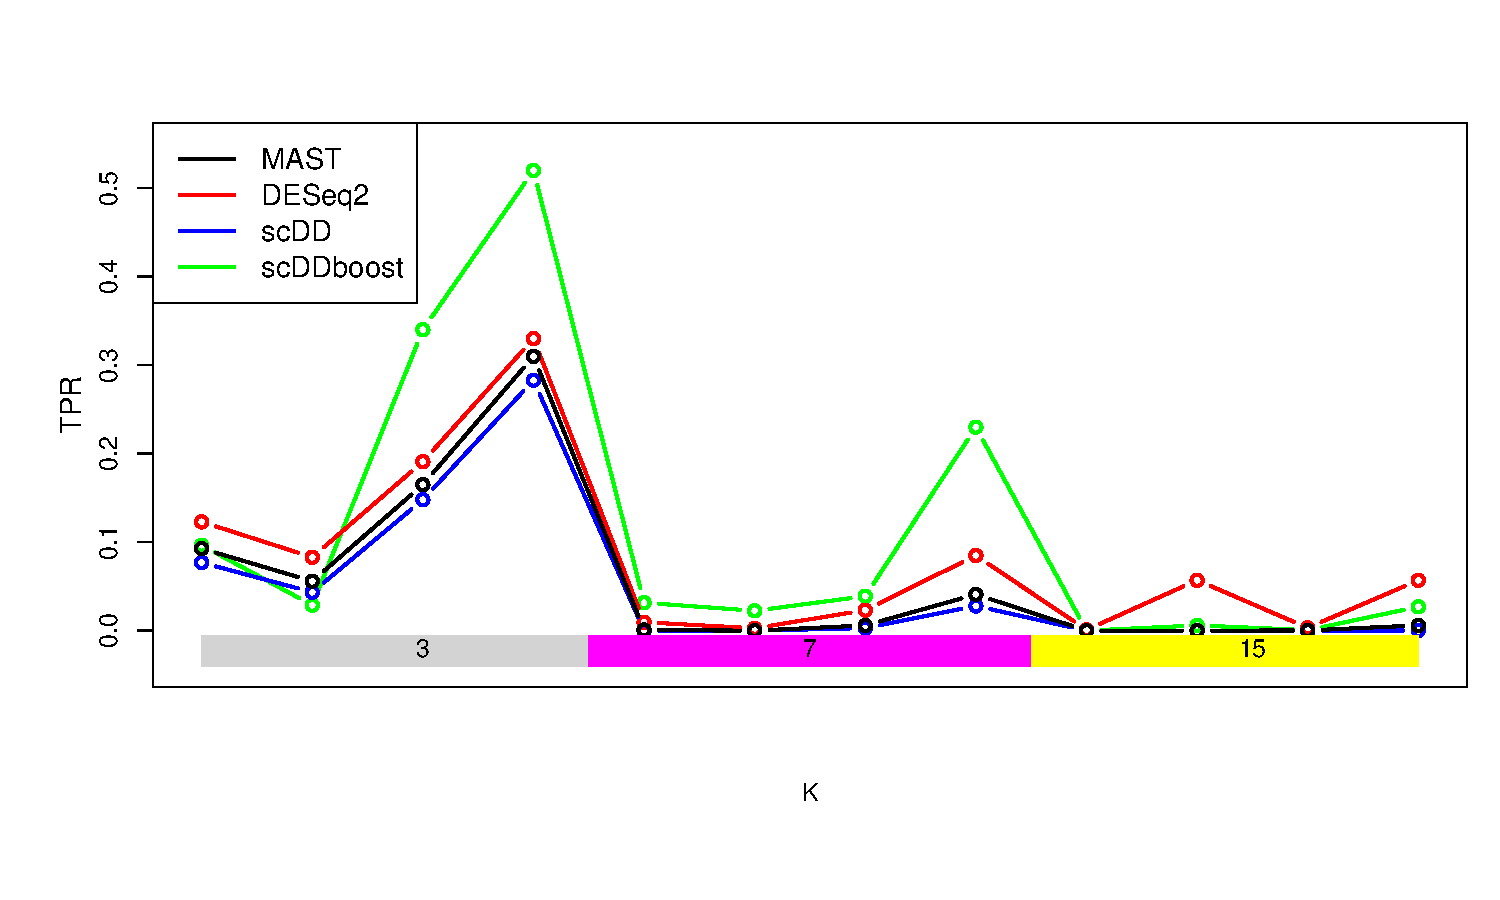
\includegraphics[width = 0.8\textwidth]{Figs/simuTPR.pdf}
  \caption{True positive rate of four methods under 3 settings of number of subtypes and 4 hyper parameters govern the difference between subtypes}
  \label{fig:5}
\end{figure}


\begin{figure}[H]
  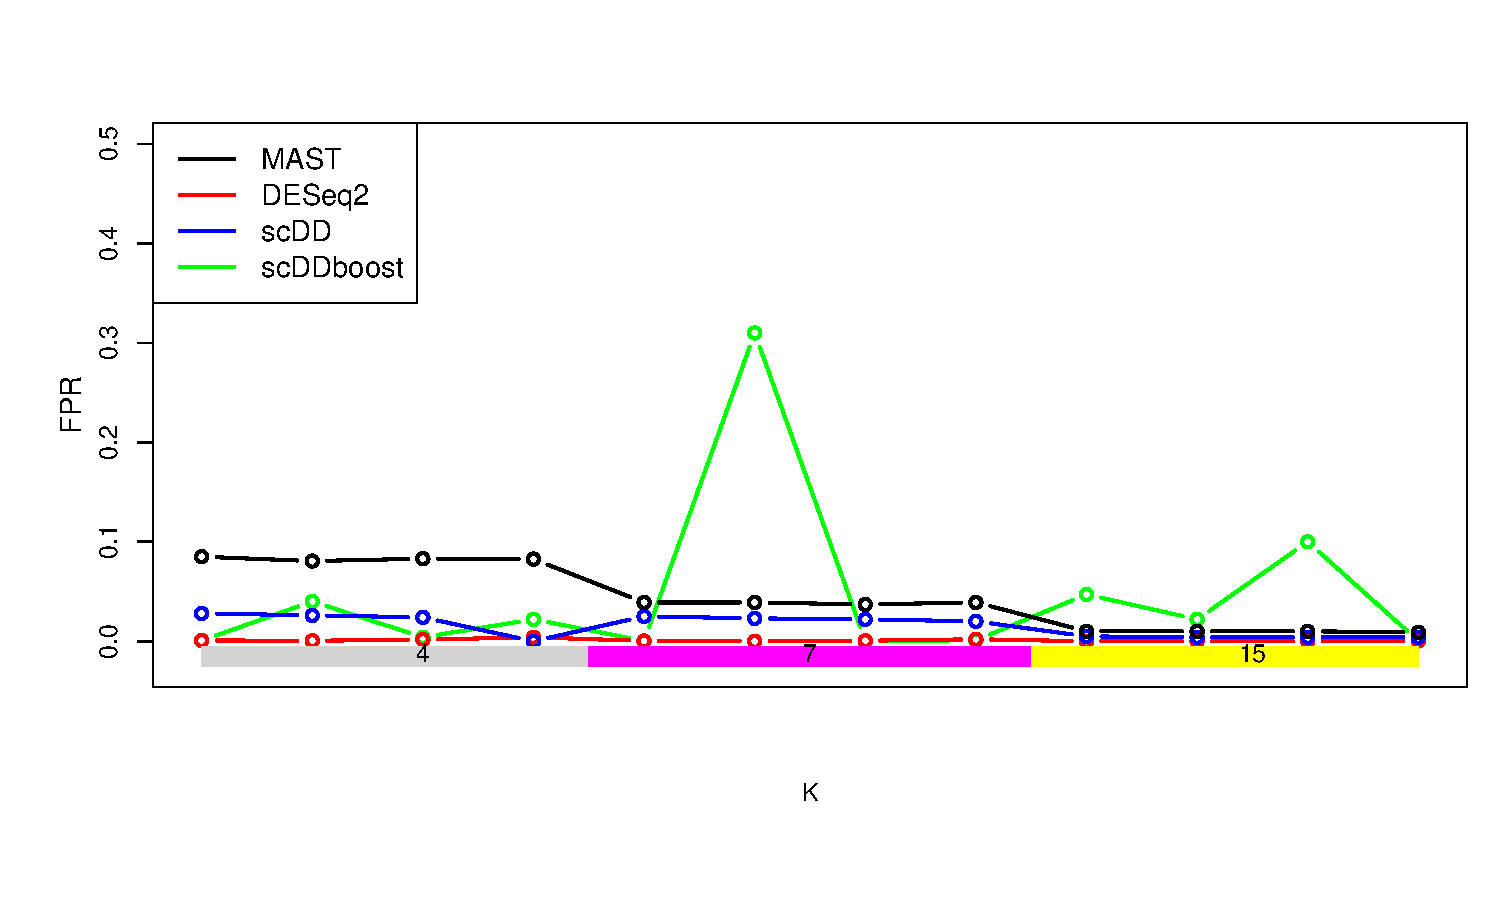
\includegraphics[width = 0.8\textwidth]{Figs/simuFPR.pdf}
  \caption{False positive rate of four methods under 3 settings of number of subtypes and 4 hyper parameters govern the difference between subtypes}
  \label{fig:5}
\end{figure}

%Since we are modeling gene transcript within each subtype as negative-binomially distributed and we only test one parameter(mean) change among subtypes. In some scenario, it could be insufficient to model the variability within subtype. Even though there is no mean expression change among subtypes but more subtle distributional change occurred among subtypes changed, EBSeq would fail to detect the discrepancies between subtypes, thus limit power of scDDboost.\\


\subsection{Empirical study}


We use 13 data sets from \verb+conquer+~\citep{ref:Cq} to test 
performance of our method on empirical data. **summarized in Supplementary Table ?** say something about
the studies **  We compare our results with 
\verb+scDD+~\citep{ref:scDD}, \verb+MAST+~\citep{ref:MAST} and 
\verb+DESeq2+~\citep{ref:Des}, 
we have also investigated performance of \verb+scDDboost+ under different clustering 
method, (\verb+sc3+~\citep{sc3}, Supplementary Table ?)  and obtain similar 

\begin{figure}[H]
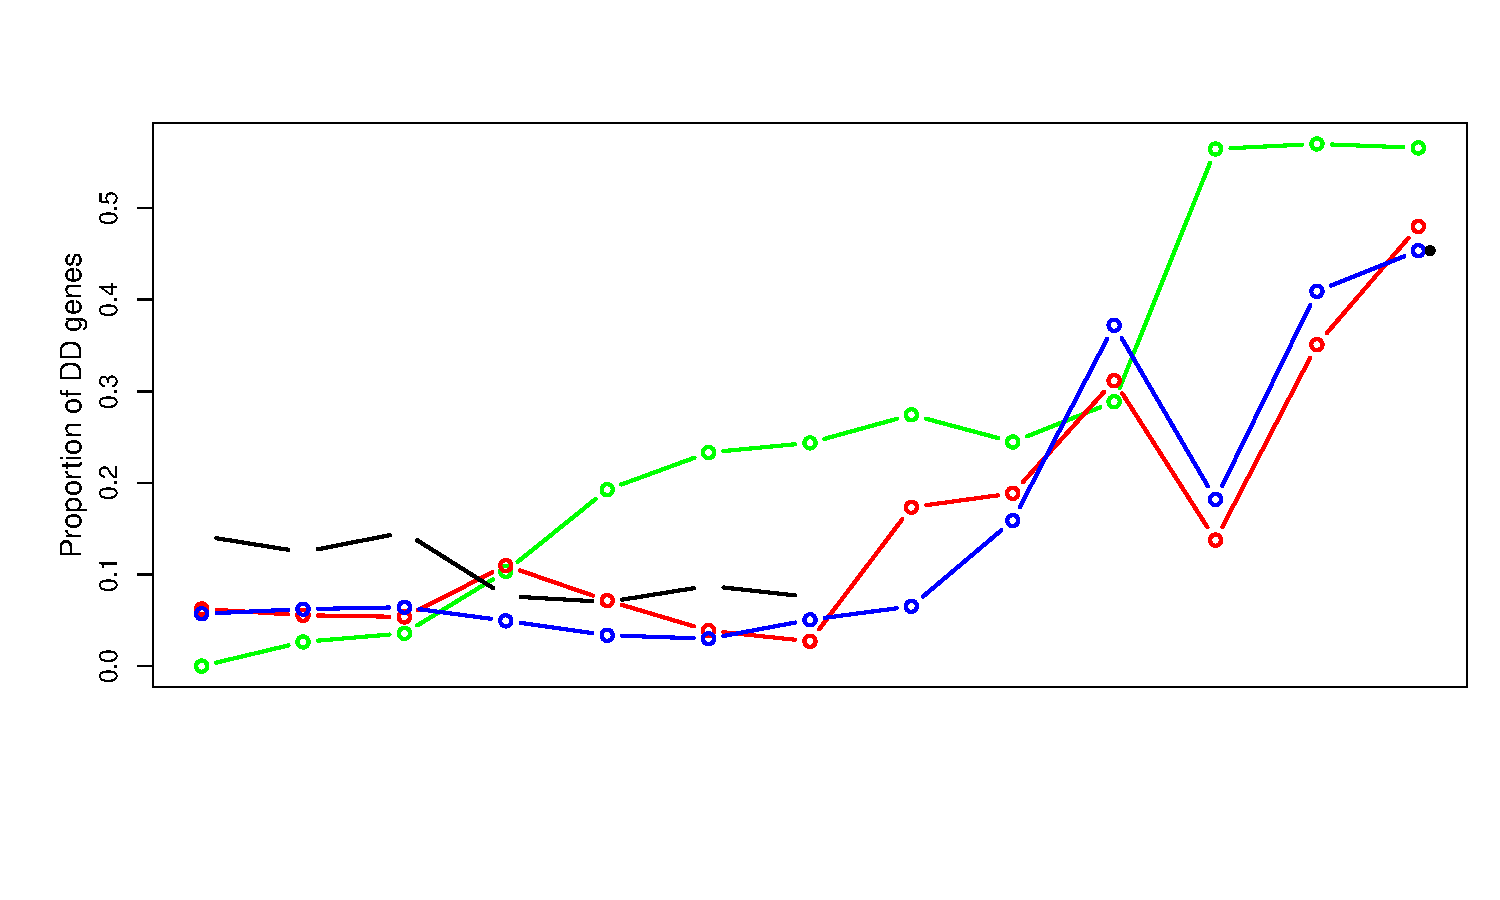
\includegraphics[width = 1\textwidth]{Figs/DD95.pdf}
 \caption{ Proportion of DD genes at 5\% threshold with respect to total number of genes identified by each method. Ranked by mean list size }
  \label{fig:6}
\end{figure}




\subsection{Null cases}

Although bulk methods seems to be the most powerful one, we found it also has a higher false discovery rate comparing to single cell methods. We validate false discovery rate on ten null datasets from table 1. For each null dataset, we randomly split the cells from one condition into two subsets and test difference of gene expression between those subsets. Since the two subsets of cells actually came from same condition, there should not be any differential distributed genes, any positive call would be a false positive. We repeat the random split and testing for five times on each null data set. We evaluate the type I error control for the methods returning nominal p-values, by recording the fraction of genes(with a valid p-value) that are assigned a nomial p-value below 0.05 (Fig 6).\\
scDDboost could control FDR since we assume cells are sampled from population composed of different subtypes. Cells from one subtype are equal likely to be assigned to either one of the two subsets. Consequently, it is very likely that proportions of subtypes remain unchanged among the two subsets.


\begin{figure}[H]
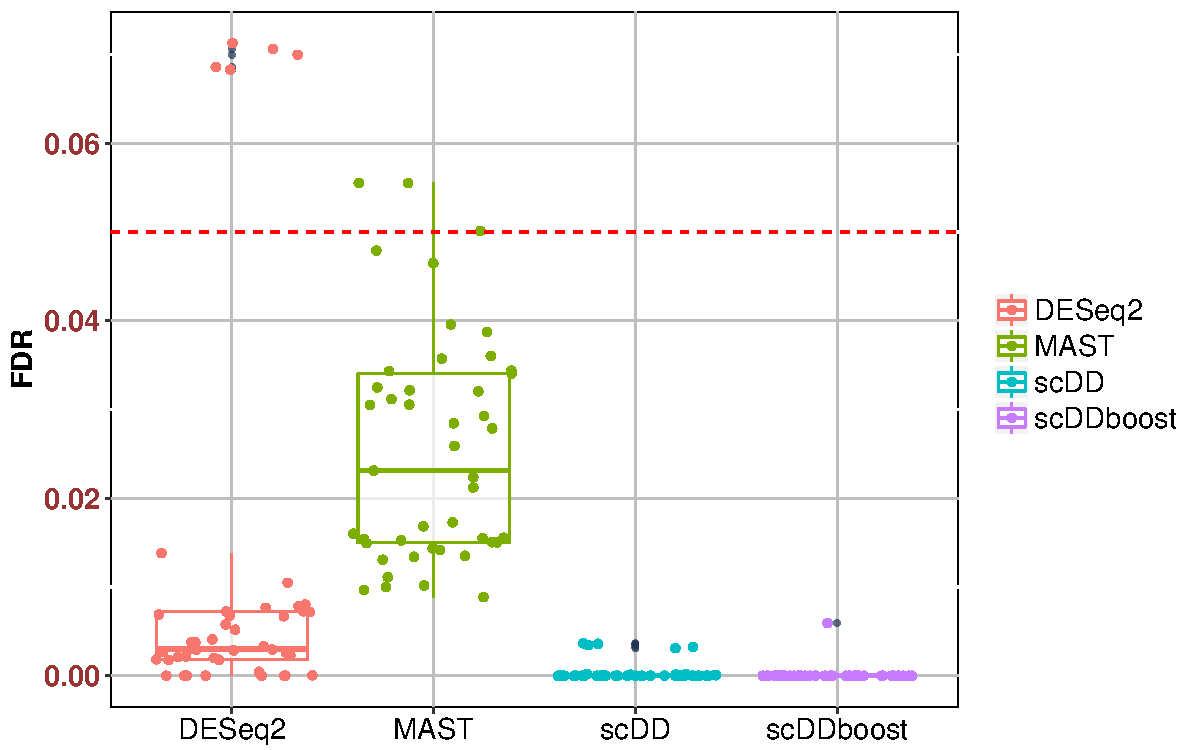
\includegraphics[width = 0.7\textwidth]{Figs/fdr.pdf}
 \caption{False positive rate of scDDboost, scDD, MAST and DESeq2 on null dataset from table 1, DESeq2 usually identify a lot but may lose the control of type I error. While other single cell methods could control FDR. }
  \label{fig:7}
\end{figure}

Number of subtypes $K$ is a crucial factor controlling the accuracy of our modeling. 
Too small $K$ may end up in an underfit such that cells within same subtype can still be very different,
mean expression change among subtypes is incapable to capture the distribution change for some genes and consequently reducing the power of \textsc{scDDboost}.
Too big $K$ may end up in an overfit such that two subtypes can be very similar, given we have fixed number of samples (cells), allowing more clusters will introduce may patterns (both for mean expression change and proportion change) to infer. Also notice the limitation of DDM model (see section 4), overestimating $K$ in \textsc{scDDboost} may losing FDR control (Fig7).

\begin{figure}[H]
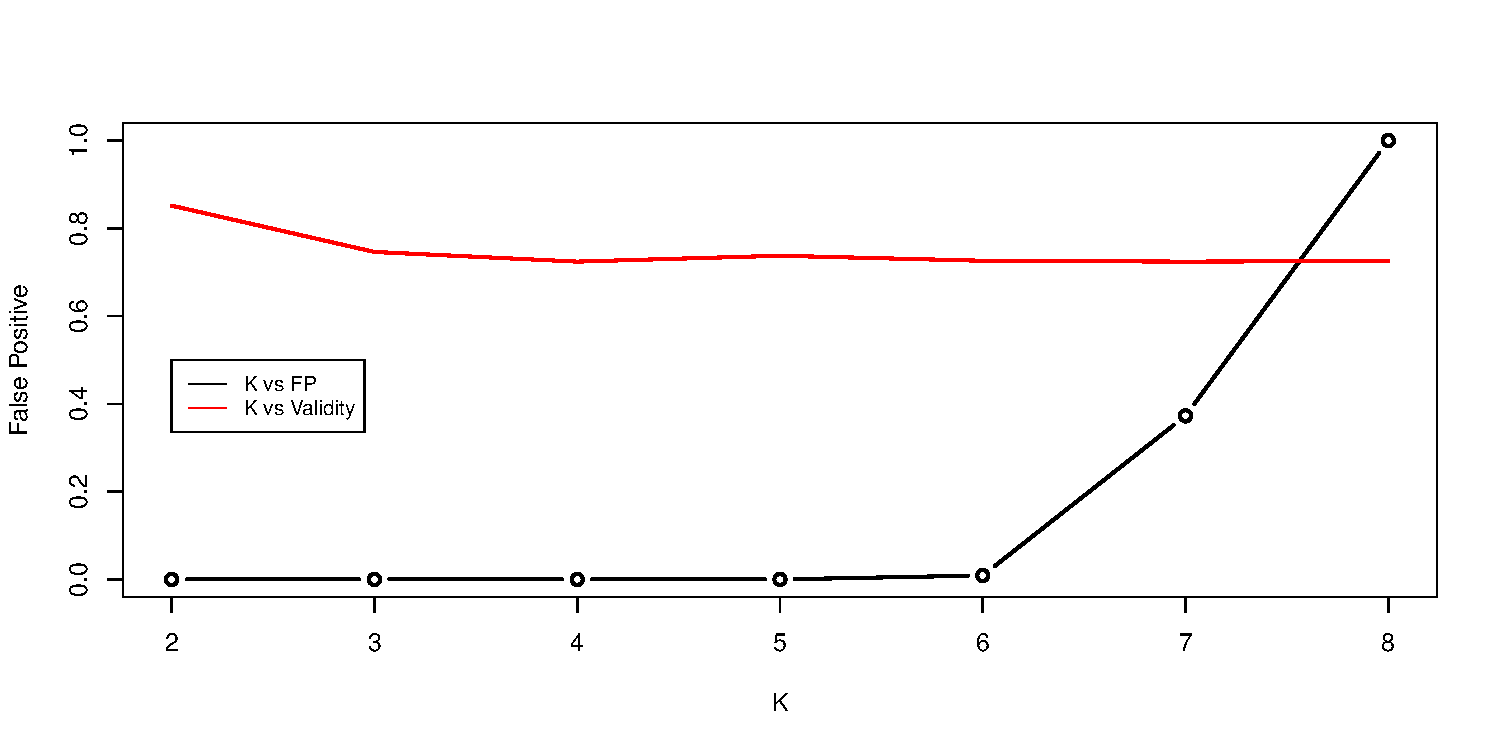
\includegraphics[width = 0.7\textwidth]{Figs/NULL.pdf}
 \caption{under NULL case, using dataset GSE52529, when using too big $K$ we may completely lose FDR control (black line shows proportion of false positive identified by scDDboost under 0.05 threshold, while validity score become stable at $K$ = 3 }
  \label{fig:7}
\end{figure}

***something about change of PDD over K, even though PDD is monotone increasing but it would remain stable in the sense that $\text{PDD}_{K+1} - \text{PDD}_K$ will have small variance over different genes***



\subsection{Bursting}

***on the method estimated p-value, update later***

D3E\citep{ref:d3e} is a distributional method that can identify bursting parameters of transcripts. Rate of promoter activation, rate of promoter inactivation and the rate of transcription when the promoter is in the active state are estimated by D3E.  We investigate DD genes identified by scDDboost and their change of those three parameters on dataset GSE71585\\

\begin{figure}[H]
%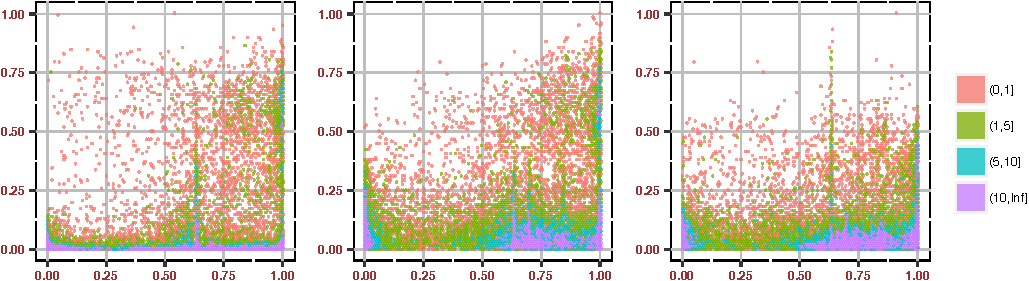
\includegraphics[width = 1\textwidth]{Figs/d3eplot.pdf}
%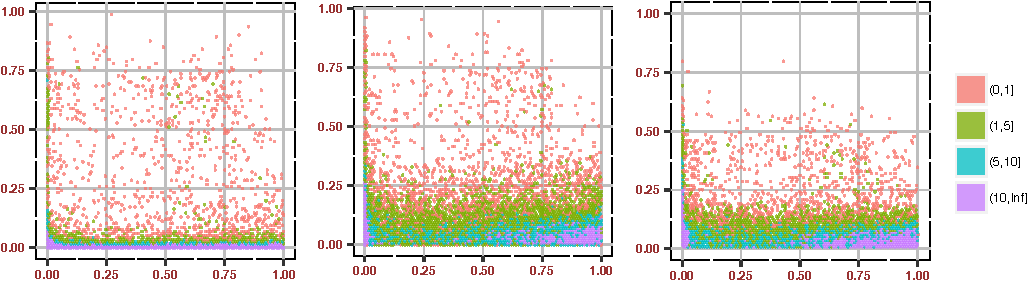
\includegraphics[width = 1\textwidth]{Figs/d3eplotdes.pdf}
%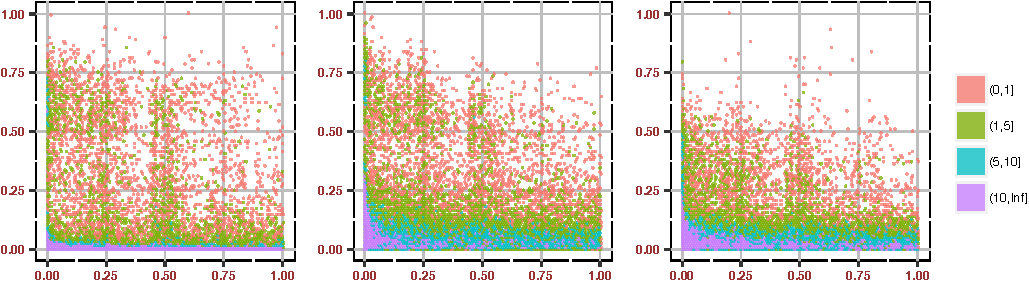
\includegraphics[width = 1\textwidth]{Figs/d3eplotmast.pdf}
%\includegraphics[width = 1\textwidth]{Figs/d3eplotscdd.pdf}
\caption{D3E method will estimate 3 bursting parameters probability of a gene being on (\textbf{a}) and off (\textbf{b}) and the expression rate when the gene expression is on (\textbf{c}), we plot the hexbin plot of probability of a gene being DD under out method v.s. the absolute value of log fold change of \textbf{a} , \textbf{b} and \textbf{c}  across the two conditions accordingly. The log fold change is scaled by dividing the largest log fold change so that ends up in a value between 0 and 1 Here we use the GSE71585 data }
\end{figure}



\begin{figure}[H]
\vspace{-\parskip}
\minipage{0.33\textwidth}
  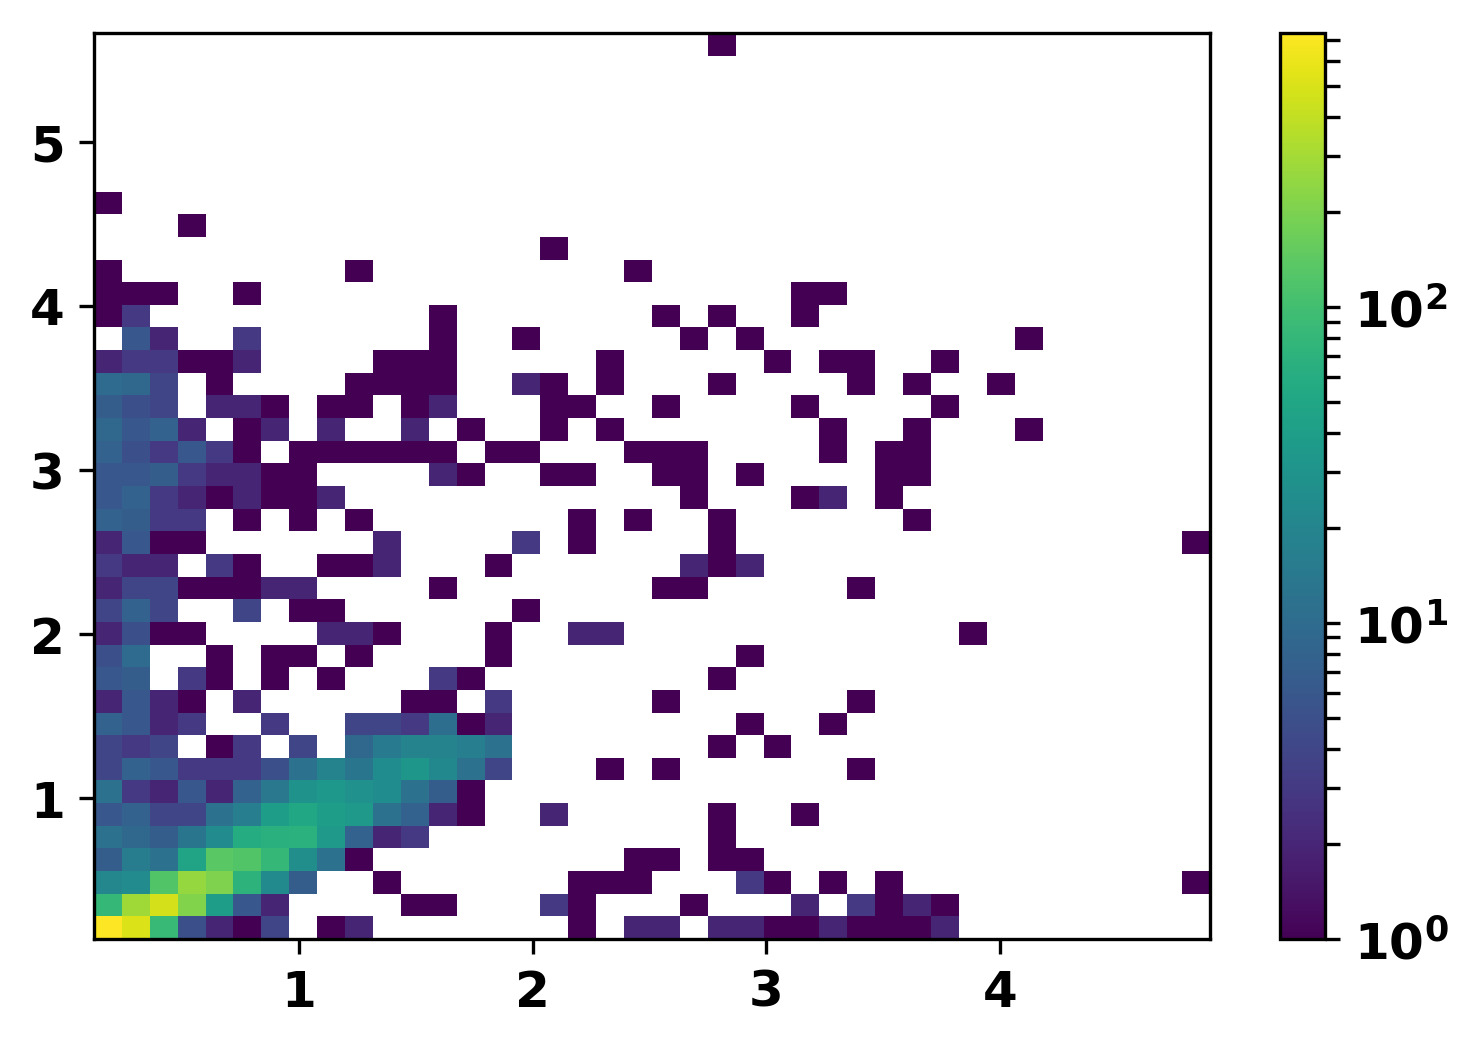
\includegraphics[clip,width=\textwidth]{Figs/act.png}
\endminipage
\minipage{0.33\textwidth}
  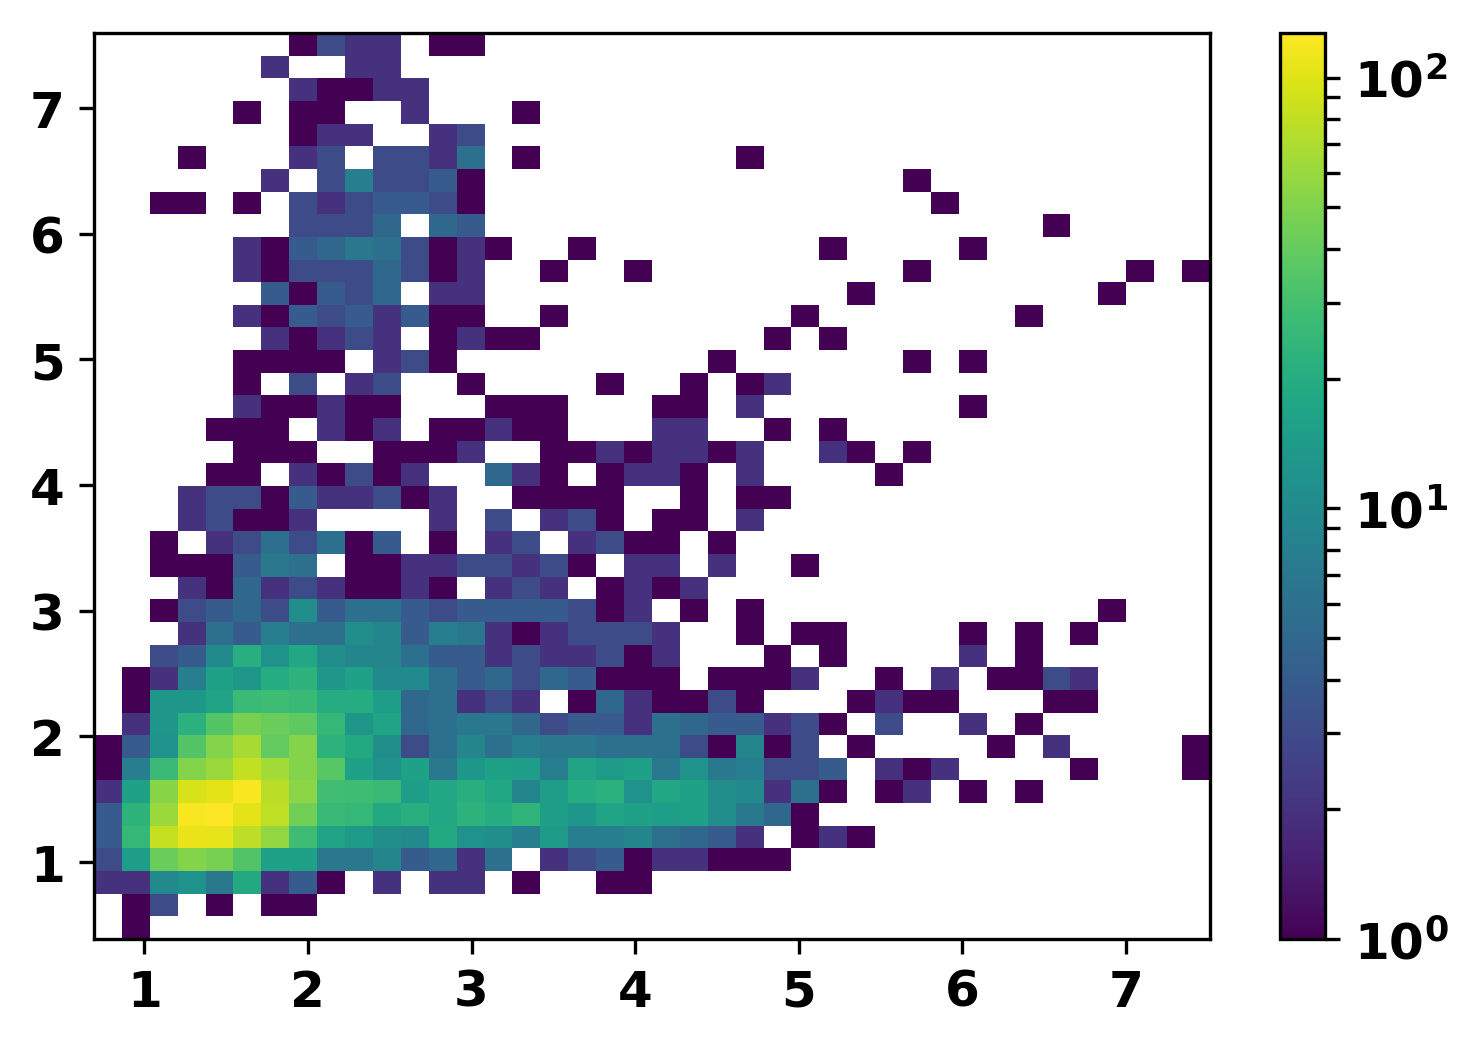
\includegraphics[clip,width=\textwidth]{Figs/in_act.png}
  \endminipage
 \minipage{0.33\textwidth}
  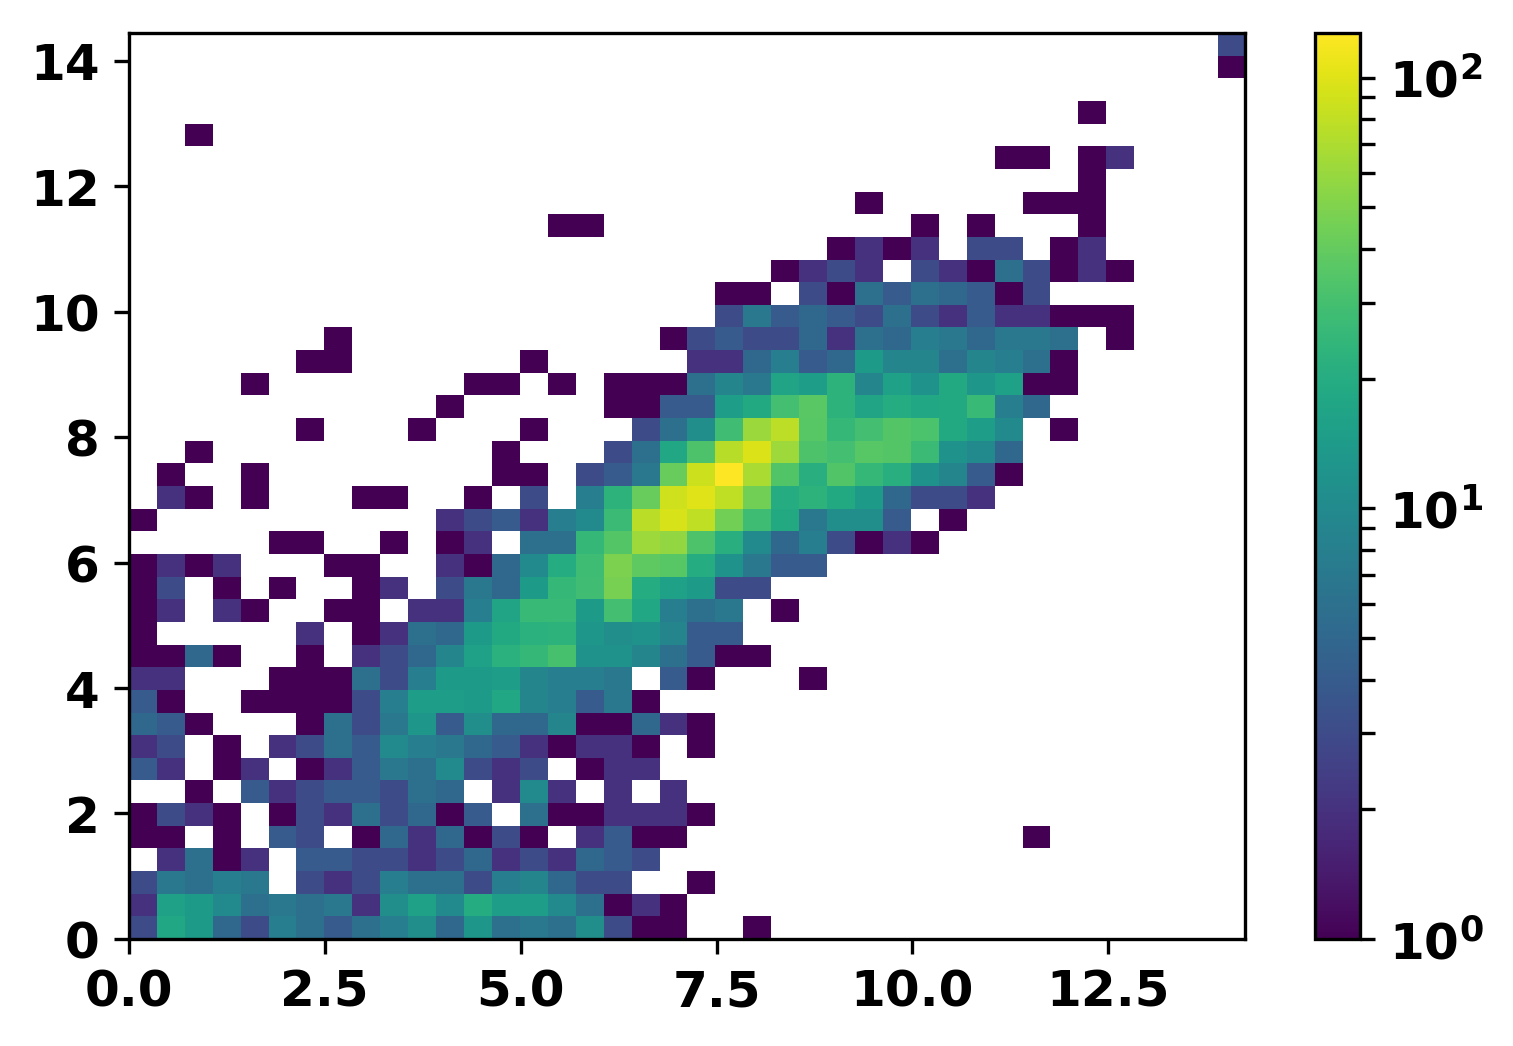
\includegraphics[clip,width=\textwidth]{Figs/t_rate.png}
  \endminipage
\captionof{figure}{2D histogram for bursting parameters of DD genes identified by scDDboost from dataset EMTAB2805 estimated by D3E. Left panel  : comparison of rate of promoter activation between two conditions, similarly, middle panel  : rate of promoter inactivation and right panel: rate of transcription when the promoter is in the active state. We observe that difference between transcription rate is smaller compare to difference between the activation and inactivation rate.}
\end{figure}

We observed that DD genes identified by scDDboost tends to have similar transcription rate when the promoter is active across condition, while there are lots of variabilities in the action and inactivation rate. Estimations from D3E reveals that the major factor to drive DD genes are activation and inactivation rate (proportions of different subtyps), it make sense to consider mixture model like scDDboost.



\section{Theoretical issues}
\subsection{Posterior consistency}
Under some parameters settings, the double dirichlet prior will have limited resolution and lead to inconsistency of posterior probabilities, which we investigate with the following asymptotic analysis.

We first give the expression of posterior probability. Since there is no information favorable of any particular $A_\pi$, we select discrete uniform distribution as the prior for it, then the posterior probability is
\begin{align}
p(A_\pi | t^1, t^2) = c*\sum_{\pi' \text{ refines } \pi} p(t^1 | t^1_{\pi'})\, p(t^2 |  t^2_{\pi'} )
 \, p( t^1_{\pi'}, t^2_{\pi'} | A_{\pi'} )
\end{align}
for a normalizing constant $\frac{1}{c} = \underset{\pi' \in \Pi}\sum p(t^1 | t^1_{\pi'})\, p(t^2|  t^2_{\pi'} )
 \, p( t^1_{\pi'}, t^2_{\pi'} | A_{\pi'} )$.
 
Let $\Omega = \{(\phi, \psi): \overset{K}{\underset{i = 1}\sum}\phi_i = \overset{K}{\underset{i = 1}\sum}\psi_i = 1, \phi_i \geq 0, \psi_i \geq 0 , i = 1,..., K\}$ be the whole space. There is a subset of $\Omega$ we lack posterior inference. Let us first see an example:
\begin{figure}[h]
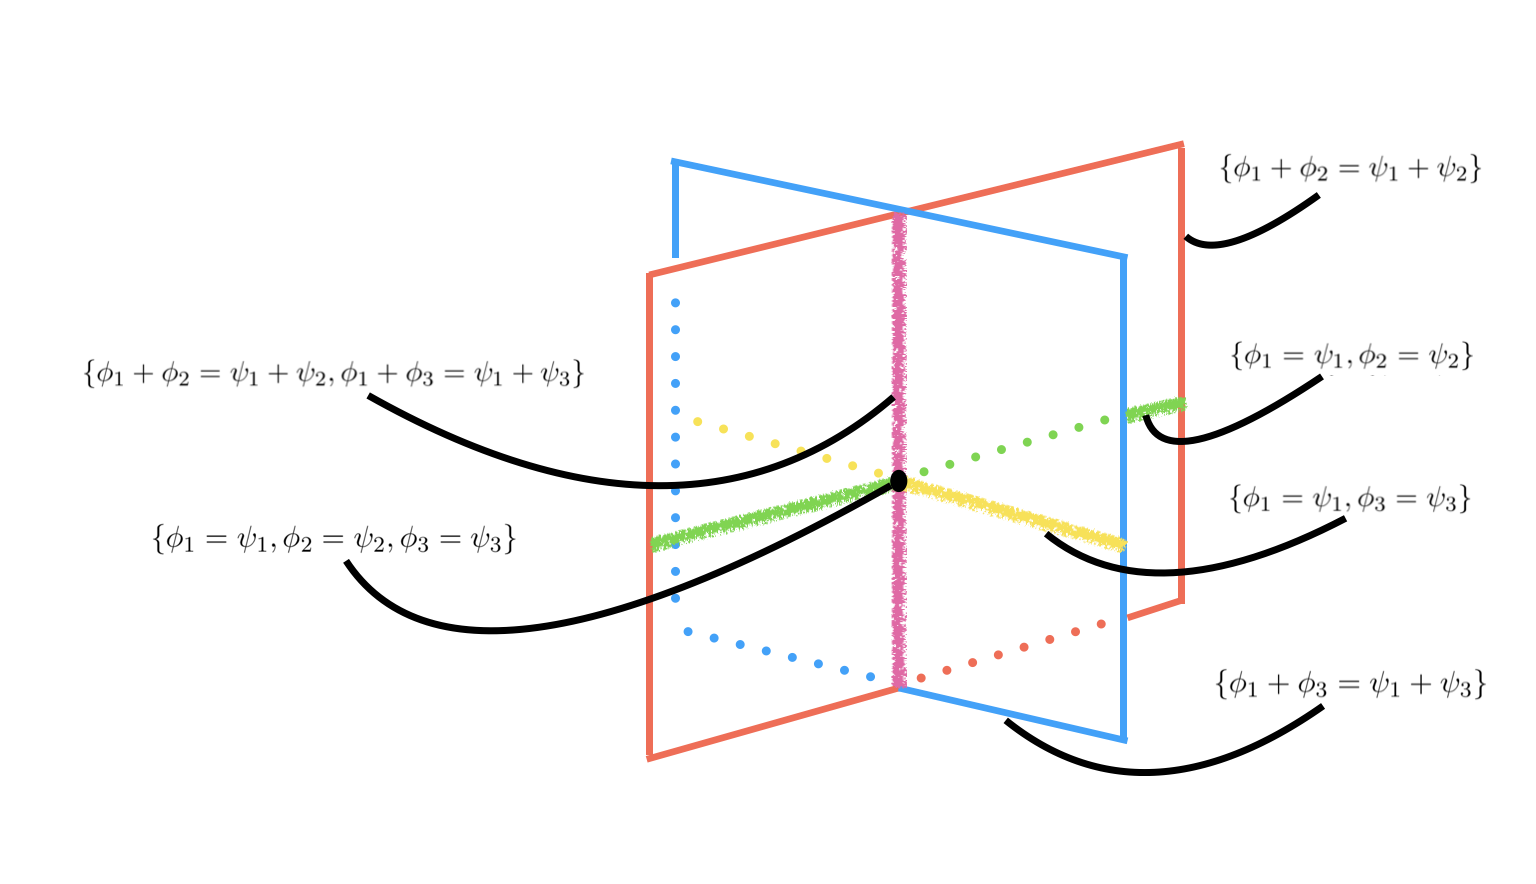
\includegraphics[scale = 0.5]{Figs/overlap.png}
 \caption{Four subtypes of cells,  simplexes of $(\phi,\psi)$ satisfying different constraints.}
  \label{fig:1}
\end{figure}
\hfill\\
In Fig 10, there are four subtypes, the rectangle with magenta boundary is a simplex $A_{\pi_1} = \{(\phi,\psi) : \phi_1 + \phi_2 = \psi_1 + \psi_2\}$, the rectangle with blue boundary is a simplex $A_{\pi_2} = \{(\phi,\psi) : \phi_1 + \phi_3 = \psi_1 + \psi_3\}$. The green line refers to $A_{\pi_3} = \{(\phi,\psi) : \phi_1 = \psi_1, \phi_2 = \psi_2\}$, the yellow line refers to $A_{\pi_4} = \{(\phi,\psi) : \phi_1 = \psi_1, \phi_3 = \psi_3\}$, the purple line refers to $A_{\pi_5} = \{(\phi,\psi) : \phi_1 + \phi_2 = \psi_1 + \psi_2, \phi_1 + \phi_3 = \psi_1 + \psi_3\}$, which is the intersection of $A_{\pi_1}$ and $A_{\pi_2}$, and finally the black dot which is the intersection of those three lines refers to the simplex with finest partitions, $\phi_i = \psi_i, \forall i = 1,..,4$. We lack posterior inference for $(\phi,\psi)$ along the purple line except the black dot. While on the green line, yellow line and black dot, we have consistent posterior inference(theorem 2). To explain why some space lacking posterior inference and define such space, we define a special subset $A_\pi^*$ of simplex $A_\pi$. $A_\pi^* = A_\pi\setminus \underset{\tilde{\pi} \text{ is not coarser than } \pi }\cup A_{\tilde{\pi}}$, $A_\pi^*$ is obtained by removing all intersection with other $A_{\tilde{\pi}}$(excluding those $A_{\tilde{\pi}}$ that is superset of $A_\pi$) from $A_\pi$. Since we removed those intersection parts. It is intuitive that $A_\pi^*$ will be disjoint subsets of $\Omega$.\\
\begin{prop}
if $\pi_1 \neq \pi_2$, then $A_{\pi_1}^*\cap A_{\pi_2}^* = \emptyset$
\end{prop}
\hfill\\
Let $Q = \Omega\setminus \underset{\pi\in \Pi}\cup A_\pi^*$, and we have following proposition of the existence of $Q$.
\begin{prop}
Let $K$ be number of subtypes. When $K >  3, Q \neq \emptyset$, when $K \leq 3, Q = \emptyset$
\end{prop}
\hfill\\
When the number of subtypes is bigger than three, we lack posterior inference on $Q$. To see that we can rewrite $A_\pi^*$ as $A_\pi^* = A_\pi\setminus \underset{\tilde{\pi} \text{ is not coarser than } \pi }\cup (A_{\tilde{\pi}}\cap A_\pi)$, $\tilde{\pi}$ is not coarser than $\pi$, which is equivalently to say $\pi$ is not refinement of $\tilde{\pi}$. By property 8 in section 2, $A_{\tilde{\pi}}\cap A_\pi$ is a lower dimensional subset of $A_\pi$. So $A_\pi \setminus A_\pi^*$ is a lower dimensional subset of $A_\pi$. For posterior on $Q$, it degenerates to integral on a lower dimensional subset of the simplex associating with densities, which will vanish\\
\begin{prop}
When $K >  3$, $p(Q | z^1, z^2) = 0$
\end{prop}
\hfill\\
But for $(\phi, \psi)\in \Omega\setminus Q$, we have consistent posterior inference. %Assuming $\alpha_i^j = 1, \forall i$ in $1,2,...,K$, $j = 1,2$ and $\beta_b = \Sigma_{i\in b} (\alpha_i^1 + \alpha_i^2) = 2N(b)$, plug in (6) and integral on $A_\pi$ then we have simplified posterior
%\begin{align}
%p(A_\pi | y,z) = \frac{1}{c'}\sum_{\pi' \in \text{RF}(\pi)}\prod_{b\in \pi'}\frac{ \Gamma(\beta_b + t_b^1 + t_b^2)}{\Gamma(N(b) + t_b^1)\Gamma(N(b) + t_b^2)} \frac{\Gamma(N(b))}{\Gamma(2N(b))}
%\end{align}
%$c'$ is the total sum over all partitions $c' = \sum_{\pi}\prod_{b\in \pi}\frac{ \Gamma(\beta_b + t_b^1 + t_b^2)}{\Gamma(N(b) + t_b^1)\Gamma(N(b) + t_b^2)} \frac{\Gamma(N(b))}{\Gamma(2N(b))} $ And we have theorem 4.\\

\begin{theorem} Let $n = min(n_1, n_2)$ be the smaller number of cells of two conditions and $n_1 = O(n_2)$ namely $\text{ln}(\frac{n_1}{n_2}) = 0$, and hyper parameters of DDM $\alpha^1, \alpha^2$ be vectors of constants, $\alpha_k^j \geq 1$, $\forall k, j$ and $\beta = \alpha^1 + \alpha^2$. Then if parameter $(\phi, \psi)\in \Omega\setminus Q $ we have 
\begin{eqnarray*}
    p(A_{\pi} | y, z) \xrightarrow[n\rightarrow\infty]{\text{a.s.}}\left\{
                \begin{array}{ll}
                 1 \quad \text{if }(\phi,\psi) \in A_\pi\\
                 0 \quad \text{otherwise}\\             
                \end{array}
              \right.
\end{eqnarray*}
\end{theorem}
\hfill\\
Things become more complicate when $(\phi, \psi)$ falling into $Q$, we know $p(Q | y, z)$ vanishes, but $p(A_\pi | y,z)$ may not. 

Recall $N(\pi)$ represents number of blocks $b$ in $\pi$. Let $S = \{\pi,  (\phi, \psi) \in A_\pi\}$, which is the collection of partitions whose associated simplexes covering $(\phi,\psi)$. Let $N^* = \underset{\pi\in S}\max$ $N(\pi)$, which is the max number of blocks of partitions from $S$. Let $S^* = \{\pi,  (\phi, \psi) \in A_\pi \text{ and } N(\pi) = N^*\}$, which is the collection of partitions that covering $(\phi, \psi)$ with number of blocks equal to the max number $N^*$. 

For example, when $K = 7$, For a $(\phi, \psi)\in A_{\pi_1} \cap A_{\pi_2} \cap A_{\pi_3}$, $\pi_1 = \{\{1,2,3\}, \{4,5,6,7\}\}, \pi_2 = \{\{1,6,7\}, \{2,4\},\{3,5\}\}, \pi_3 = \{\{1,2,3,4,5,6\}\}$, and also $(\phi, \psi)$ does not belong to any other simplex $A_\pi$. Then $S = \{\pi_1, \pi_2, \pi_3\}$, $N^* = 3$, $S^* = \{\pi_2\}.$ 

%Denote components from right hand side of (5): $\frac{1}{c'}\underset{b\in \pi}\prod\frac{ \Gamma(\beta_b + t_b^1 + t_b^2)}{\Gamma(N(b) + t_b^1)\Gamma(N(b) + t_b^2)} \frac{\Gamma(N(b))}{\Gamma(2N(b))} = J(y,z,\pi).$  We have theorem 5.\\
\begin{theorem} Following the setting in theorem 4, when parameter $(\phi, \psi)\in Q$,  and further if $\alpha^j, j = 1,2$ are vectors of integers, we have 
\begin{eqnarray*}
    (p(A_{\pi} | y, z))_{\pi\in S^*} \xrightarrow[n\rightarrow\infty]{\text{d}}%\left\{
                %\begin{array}{ll}
                (V_1, ..., V_{N(S^*)})
                 %m(\pi) \quad  \pi \in S^* \\
                 %0 \quad \text{otherwise}\\             
               % \end{array}
              %\right.
\end{eqnarray*}
%and $\underset{\pi\in S^*}\sum m(\pi) = 1, m(\pi) > 0$\\
$V_1, ..., V_{N(S^*)}$ are random variables and $V_1 + .. + V_{N(S^*)} = 1$
\end{theorem} 

Still using above example, in limiting case, we have $p(A_{\pi_3} | y,z) = 1$, $p(A_{\pi_2} | y,z) = 1$ and $p(A_{\pi_1}| y,z) = 0$. When the DE pattern is $B_{\pi_1}$ for some genes and our estimation of $p(A_{\pi_1}| y,z) = 0$, we will falsely classify those genes as differential distributed.

The asymptotic properties help us gain insight of the performance of our approach,
scDDboost may work poorly, when $(\phi, \psi)\in Q$, we may underestimate the posterior probability of true proportion change pattern, which reduce the posterior probabilities of true negative and enlarge false positive rate.\\

\subsection{Random weighting}
In this section, we gave an intuitive justification for consistency between bayesian framework clustering analysis and random weighting procedure. A full bayesian analysis for clustering needs to specify the density of data given the partition. Specifically, in single cell analysis we need to know the density of transcripts of genes given the partitions which requires understanding of co-expression and dependence between genes. Instead of trying to untangle the mystery behind the dependence of genes, we consider following approximation 

\begin{eqnarray*}
P(\text{Partition} | X) \leftarrow P(\text{Partition} | D) \leftarrow P(\Delta | D) \leftarrow D / W
\end{eqnarray*} 

where $D$ is the estimated distance matrix of $X$, $\Delta$ is the true distance of $X$ and $W$ is randomly distributed matrix of weights. We conjecture that the probability of partitions given data can be approximated by switching conditioning on data to conditioning on the estimated distance of data. As distance matrix typically gave the geometrical structure between elements which can be used to infer how likely a partition is.  In addition, partition can be obtained by  distance based clustering algorithm (K-medoids) on true distance matrix $\Delta$.  To approximate distribution $(\Delta | D)$, we use our random weighting procedure, namely sampling a weighting matrix $W$ first and then do the component-wisely dividing of original distance matrix $D$ by $W$.

We gave a brief justification for this approximation, suppose units $i$ and $j$ are merged into a common cluster if (and only if) $d_{i,j} < c$. Then $P(d^*_{i,j} < c) = P(w_{i,j} > c / d_{i,j})$, $w_{i,j} \sim$ Gamma$(a, b)$. From Bayesian perspective, given the true distance $\Delta_{i,j}$, $d_{i,j} | \Delta_{i,j} \sim$ Gamma($a_1, a_1 / \Delta_{i,j}$), so that the sampling mean of $d_{i,j}$ is $\Delta_{i,j}$.  Further, for simplicity we ignore any issues about the $d$'s or $\Delta$'s being true distances. The condition for qualifiable distance matrix is the triangle inequality among the pairwise distances, such condition would not affect our clustering results too much. But, a simple analysis might suppose that a-priori $1 / \Delta_{i,j} \sim$ Gamma($a_0, d_0$). The scaling is such that E$(1 / \Delta_{i,j}) = a_0 \ d_0$. The posterior, by conjugacy, has $1 / \Delta_{i,j} | d_{i,j} \sim$ Gamma($a_0 + a_1, d_0 + a_1d_{i,j}$). Then the posterior probability that $i$ and $j$ should be clustered is the posterior probability that $\Delta_{i,j} < c$, which is $P($Gamma($(a_0 + a_1),(a_0 + a_1)) > (d_0 + a_1 * d_{i,j}) / (a_0 + a_1) * 1/c )$, parameters $(a_0, d_0, a_1)$ are estimated from maximizing the marginal likelihood of $d_{i,j}$.

In order to match the posterior probability that elements $i$ and $j$ belongs to the same cluster through the simple bayesian analysis to random weighting, which is equivalently to match 
\begin{eqnarray*} 
P(\Delta_{i,j} < c | d_{i,j}) = P( 1 /  \Delta_{i,j} > 1 / c | d_{i,j})
\end{eqnarray*}
and 

\begin{eqnarray*}
P(d_{i,j} / w_{i,j} < c | d_{i,j}) = P(w_{i,j} / d_{i,j} > 1 / c | d_{i,j})
\end{eqnarray*}

yielding $a = a_0 + a_1$ and $b = a_1$.  Therefore, we gave a way of modeling the distribution of weights such that partition based on random generated distance $D / W$ would approximate the partition given data based on a full bayesian framework.



\section{Discussion}
We have presented scDDboost, a compositional model for detecting differential distributed genes from scRNA-seq data. To account for the over-dispersion and multi-modality of single-cell data, scDDboost modeled transcripts as mixture distributed. Unlike previous invented methods (e.g. Deseq2, MAST and scDD), which conducts genewise DD test in an isolated manner. scDDboost make whole genome information shared at gene level by further assuming the mixture distribution of transcripts is a mixture over the subtypes of cells. Another advantage of scDDboost is its' flexibility to allow user specified clustering methods of cells, with more and more studies of the scRNA-seq data, there will be more accurate distance matrix between cells, which will yield better estimation of subtypes and inference of DD genes. We combine estimations of changes of subtypes' proportions across conditions and changes of mean expressions across subtypes to infer distributional changes of transcripts. To estimate changes of subtypes' proportions across conditions, we use empirical Bayes and developed a double Dirichlet prior distribution.  We invented a random weighting scheme that stabilize our DD inference as well as approximating the results as if we have done a fully bayesian clustering analysis based on Dirichlet prior.  We demonstrated that scDDboost outperforms existing approaches in simulation and tends to be more powerful than existing methods on a wide range of public available empirical datasets. 

One limitation of scDDboost is that current EBseq inference of the DE patterns is computationally not feasible for big number of subtypes. Given the noise level among the single cell data and especially if we want to identify DD genes among conditions containing thousands of cells, allowing a big number of subtypes would make cells under same subtype more homogeneous and result in a more accurate estimations for the distribution of transcripts. Further research is needed for acceleration of EBseq, one direction is to reduce the calculation on those patterns that would have small posterior probabilities. 




%\bibliographystyle{IEEEtran}
%\bibliographystyle {plainnat}
\bibliographystyle{imsart-nameyear}
\bibliography{./references/wlr_ref}

\newpage

%%\appendix
 
\section*{Appendix}

\subsection*{Proof of Theorem 1}

If $\theta \in \bigcup_{\pi \in \Pi} \left[ A_{\pi} \cap M_{g, \pi} \right]$, then there exists a partition $\pi$
for which $\theta \in A_\pi$ and $\theta \in M_{g,\pi}$.   By construction
\begin{eqnarray*}
f^1_g(x) = \sum_{k=1}^K \phi_k f_{g,k}(x) 
         = \sum_{b \in \pi} \sum_{k \in b} \phi_k f_{g,k}(x) 
         = \sum_{b \in \pi} \Phi_b f_{g,k^*(b)}(x) ,
\end{eqnarray*}
where $k^*(b)$ indexes any component in $b$, since all components in that block have the same component distribution
owing to constraint $M_{g,\pi}$. Continuing, using the constraint $\theta \in A_{\pi}$,
\begin{eqnarray*}
f^1_g(x) = \sum_{b \in \pi} \Psi_b f_{g,k^*(b)}(x) = f^2_g(x)   \qquad \forall x.
\end{eqnarray*}
That is, $\theta \in {\mbox {\rm ED}}_g$.


If $\theta \in {\mbox {\rm ED}}_g$, then $f^1_g(x) = f^2_g(x)$ for all $x$.  Noting that both are mixtures over
the same set of components $\{ f_{g,k} \}$, let $\{ h_{g,l} : l=1,2, \cdots, L\}$ be the set of distinct 
components over this set, and so
\begin{eqnarray*}
f^1_g(x) = \sum_{k=1}^k \phi_k f_{g,k}(x)   
         = \sum_{l=1}^L c_{g,l} (\phi) h_{g,l}(x) 
         = \sum_{l=1}^L c_{g,l} (\psi) h_{g,l}(x) 
         = f^2_g(x ) 
\end{eqnarray*}
where
\begin{eqnarray}
\label{eq:cprobs}
c_{g,l}(\phi) = \sum_{k=1}^K \phi_k 1[ f_{g,k} = h_{g,l} ]   \qquad
c_{g,l}(\psi) = \sum_{k=1}^K \psi_k 1[ f_{g,k} = h_{g,l} ]  .
\end{eqnarray}
Finite mixtures of distinct negative binomial components are identifiable (Proposition~5 from ~\cite{yak68}), 
and so the equality
of $f^1_g$ and $f^2_g$ implies $c_{g,l} (\phi) = c_{g,l} (\psi)$ for all $l=1,2, \cdots, L$.  
Identifying the partition blocks $b_l = \{ k: f_{g,k} = h_{g,l} \}$, and the partition $\tilde \pi = \{b_l\}$,
we find $\theta \in A_{\tilde \pi} \cap M_{g, \tilde \pi}$. The accumulated probabilities in~(\ref{eq:cprobs})
correspond to $\Phi_{\tilde \pi}$ and $\Psi_{\tilde \pi}$, which are equal on $A_{\tilde \pi}$.


\subsection*{Pseudo-code}

\begin{algorithm}
\caption{\textsc{scDDboost}}\label{alg:scDDboost}
\raggedright\hspace*{\algorithmicindent} \textbf{Input}: \begin{list}{}{}
 \item  \textsc{genes} by \textsc{cells} expression data matrix $X=(X_{g,c})$
 \item  cell condition labels $y=(y_c)$
 \item  number of cell subtypes $K$
 \item number of randomized clusterings $n_r$
 \end{list}
\hspace*{\algorithmicindent} \textbf{Output}: posterior probabilities of differential distribution
\begin{algorithmic}[2]
\Procedure{scDDboost}{$X,y, K, n_r$}
\State distance matrix: $D=\rm{dist}(X) \gets$ pairwise distances between cells (columns of $X$)
\State hyper-parameters $(\hat a, \hat b) \gets {\mbox {\rm hyper}}(D)$
\Repeat
\State Gamma noise vector: $e$, with components $\sim \text{Gamma}(\hat a,\hat b)$
\State randomized distance matrix: $D^* \gets D / (e\textbf{1}^T +  \textbf{1}e^T)$
\State $\hat z^* \gets {\mbox {\rm $K-$medoids}}(D^*)$
\State $P^* \gets\;$ \textsc{scDDboost-core}$(X,y,\hat z^*)$
\Until{$n_r$ randomized distance matrices}
\State \textbf{return} $\forall \text{genes} \, g, \, P(\text{DD}_g|X,y) = \frac{1}{n_r}
   \sum_{D^*} P^*_g$
\EndProcedure
\end{algorithmic}
\end{algorithm}





\end{document}  
